\chapter{Background}

\section{Wireless Communications}

This section aims to provide a general overview of relevant wireless communication terminology and other principles necessary to understand the more hardware-oriented part of this thesis.

\subsection{Problems with established wireless communication techniques}

\begin{figure}[htbp]
    \centering
    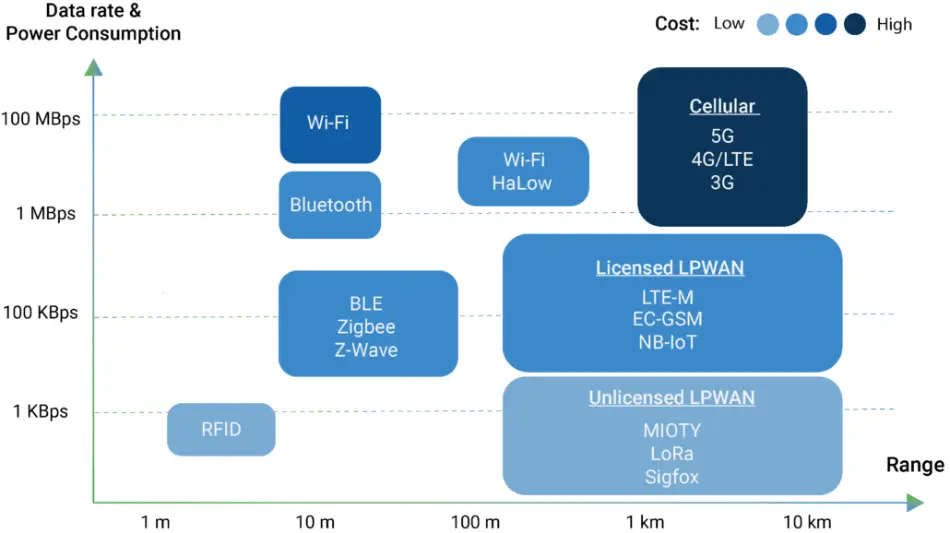
\includegraphics[width=1\textwidth]{pictures/lora/comparison-wireless-protocols.png}
    \caption[Comparison of data rate, power consumption and range between different wireless communication protocols.]
        {
            Comparison of data rate, power consumption and range between different wireless communication protocols.
            While \ac{LoRaWAN} has significantly lower data rates compared to cellular networks, its power consumption and cost is also much lower.~\protect\cite{wang_comparison_2021}
        }\label{pic:wireless-protocols-comparison}
\end{figure}

While there are sensors that can be connected to the internet using Wi-Fi, ZigBee, \ac{LTE} and other, these technologies are not suitable for all use cases.

Sensors deployed in remote or large areas may be inaccessible or separated by several hundred meters, necessitating the use of
long-range links for deployments in these regions.
This makes low power sensors that can run on batteries for several months to years a necessity, as battery replacement can be expensive or even impossible.

For instance, Wi-Fi is unsuitable for battery-powered \aclp{ED} in remote areas, both because it requires relatively high power to operate and has a limited range.
Similarly, ZigBee's limited range makes it unsuitable for remote locations.
While \ac{LTE} has a rather large range, is also unsuitable for battery powered \aclp{ED} either as it requires a lot of power.
A rough comparison between selected wireless protocols can be seen in \Cref{pic:wireless-protocols-comparison}~\cite{wang_comparison_2021}.

\subsection{Comparing signal strengths — \acl{RSSI}}\label{sec:rssi}

The \acf{RSSI} is a measure of the strength of the wireless signal strength as received by a receiver.
As far as this thesis is concerned, \ac{RSS} values are measured in dBm since the \ac{TTN} \ac{LNS}, the basis for all data used, uses this unit as well~\cite{the_things_industries_bv_data_2023}.

Different \aclp{ED} can have different \ac{RSS} values for the same distance because of factors such as antennas with different gains.
Furthermore, \ac{RSS} values can only function reliably when there is nothing blocking the signal between the transmitting and receiving stations, e.g.,\ if there is a \ac{LoS} between the sender and receiver.
The \ac{RF} signal may be obstructed and weakened by structures, trees, or other physical barriers.
This is due to a phenomenon known as \acf{MPP} which will later be explained in \Cref{sec:multipath-propagation}~\cite{kucherov_investigation_2021}.

\subsubsection{Correlation between \acs{RSS} values and distance — \acf{FSPL}}\label{sec:background-free-space-path-loss}

Usually, the higher the \ac{RSS} value, the closer the sender is to the receiver since the signal is stronger when the radio waves have to travel a shorter distance~\cite{stutzman_antenna_1981}.
When using two non-directional (isotropic) antennas, there is a certain correlation between the distance between sender and receiver and the \ac{RSSI} value.

The equation to calculate this so-called \acl{FSPL} in decibels can be seen in \Cref{eq:fspl}~\cite[p. 1321]{whitaker_electronics_1996}.

\begin{equation}\label{eq:fspl}
    FSPL_{dB} = 20 \log_{10}\left(\frac{4 \pi d}{\lambda}\right)
\end{equation}

$d$ is the distance between sender and receiver, while $\lambda$ is the wavelength of the signal.

\begin{equation}\label{eq:wavelength-of-a-signal}
    \lambda = \frac{c}{f}
\end{equation}

To calculate the wavelength of a signal, the formula seen in \Cref{eq:wavelength-of-a-signal} is used, where $\lambda$ is the wavelength, $c$ is the speed of light, and $f$ is the frequency.
As the \ac{LoRa} modulation operates at \SI{868}{\mega\hertz} in the \ac{EU}, its wavelength can be calculated as $\lambda = \frac{299792458 \text{ m/s}}{868 \times 10^6 \text{ Hz}} \approx 0.345 \text{ m}$~\cite{lora_alliance_inc_lorawan_regional_2017}.

As an example, the \acl{FSPL} in \si{\decibel} for a distance of \SI{1}{\kilo\metre} (\SI{1000}{\metre}) with the \ac{LoRa} frequency can be calculated as follows: $20 \log_{10}\left(\frac{4 \pi \times 1000}{0.345}\right) \approx 91.23 \text{ dB}$.

\subsubsection{Influences of external factors on \acs{RSS} — \acl{MPP}}\label{sec:multipath-propagation}

In addition to a signal reaching its destination directly, a \ac{RF} transmission phenomenon called \acf{MPP} can occur.
\acl{MPP} can cause the \ac{RSS} values to fluctuate even when neither the distance between the transmitter and receiver nor their antennas change~\cite[p. 136]{abdelfadeel_how_2019}.

\begin{figure}[htbp]
    \centering
    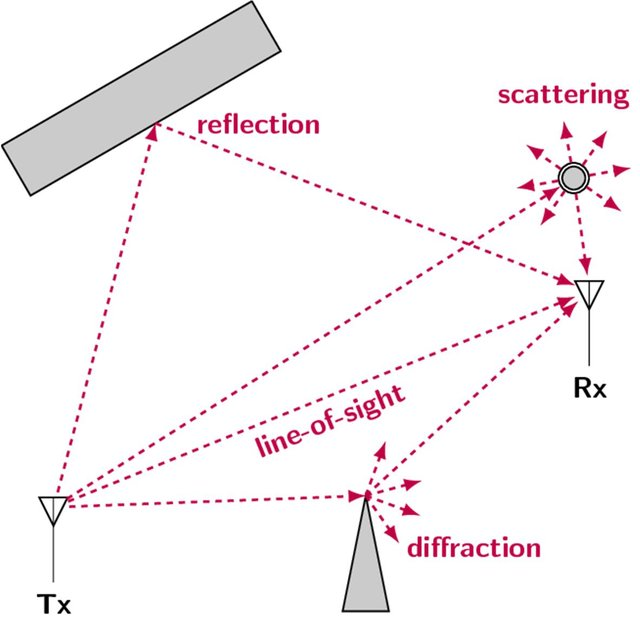
\includegraphics[width=0.4\textwidth]{pictures/diagrams_figures/multipath_propagation.jpg}
    \caption[Examples for different types of \acl{MPP} effects of \acl{RF} waves.]{
        Examples for different types of \acf{MPP} effects of \ac{RF} waves.
        Notably, all of them make the signal's travel time longer than a direct \ac{LoS} path would take.
        This longer travel time in turn also decreases the \ac{RSS} value measured by the receiver.~\protect\cite{milosevic_key_2017}
    }\label{pic:figure_multipath_propagation}
\end{figure}

This is because the signal can be reflected, diffracted, refracted and scattered, taking multiple paths (hence the term \acl{MPP}) as shown in \Cref{pic:figure_multipath_propagation}.

\subsection{Describing influences of noise on the signal — \acf{SNR}}\label{sec:background-snr}

Since the \SI{868}{\mega\hertz} frequency band used for \ac{LoRa} in the \ac{EU} is unlicensed, it is possible that other devices use the same frequency band~\cite{etsi_etsi_2012}.
This can result in a relatively high level of so-called radio noise~\cite[p. 6]{fujdiak_insights_2022}.

The \acf{SNR} is a measure of the strength of the signal compared to the noise in the signal~\cite{johnson_signal--noise_2006}.
Its formula is as follows:

\begin{equation}
    \text{SNR} = \frac{P_{Signal}}{P_{Noise}}
\end{equation}

A \ac{SNR} of 1 means that the signal and the noise are equally strong.
While a \ac{SNR} above 1 indicates a signal that is stronger than the noise, a \ac{SNR} below 1 indicates a signal that is weaker than the noise.
The \ac{SNR} can be impacted by several environmental factors, such as the temperature and humidity of the air~\cite{jeftenic_impact_2020}.
While the \ac{SNR} can also be expressed in \si{\decibel}, in this thesis it is expressed as a ratio because \ac{TTN} uses that format.

\section{Terminology: \acs{LoRa} vs. \acs{LoRaWAN}}

\acf{LoRa} is a \ac{RF} communication modulation that offers a standardized way to send data packets over the air in a specific way~\cite{semtech_corporation_lora_2023}.
A rough explanation of its technical details will be given in \Cref{sec:lora-modulation}.

\ac{LoRaWAN} is a network protocol that uses \ac{LoRa} as its physical layer to transmit data packets.
It will be explained in more detail in \Cref{sec:lorawan}.

\section{The \acs{LoRa} modulation}\label{sec:lora-modulation}

The \ac{LoRa} modulation, also known as ``\ac{LoRa}\ PHY'', enables long-range communication with low power consumption~\cite{chaudhari_understanding_2022}.
In the \ac{EU}, it operates mostly on the \SI{868}{\mega\hertz} frequency band to transmit data~\cite{lora_alliance_inc_lorawan_regional_2017}.
This frequency spectrum was utilized exclusively for the experiments conducted in this thesis.

This section will explain some of its concepts that are relevant to this thesis.
However, it will not go into detail about all technical details of the modulation.

\subsection{Transmitting \acs{LoRa} signals with resilience to interference with \acf{CSS}}\label{sec:chirp-spread-spectrum}

\ac{LoRa} uses a technique called \acl{CSS} to transmit data with the possibility for error detection and correction~\cite{reynders_chirp_2016}.
\acs{CHIRP} stands for \acl{CHIRP}.
It uses frequency hopping and different \aclp{SF} to encode signals in order to make them robust against interference, as will be explained in \Cref{sec:spreading-factors}.

\subsection{Regio-specific parameters for the \acs{LoRa} modulation in the \acs{EU} region}\label{sec:duty-cycle}

\begin{figure}[htbp]
    \centering
    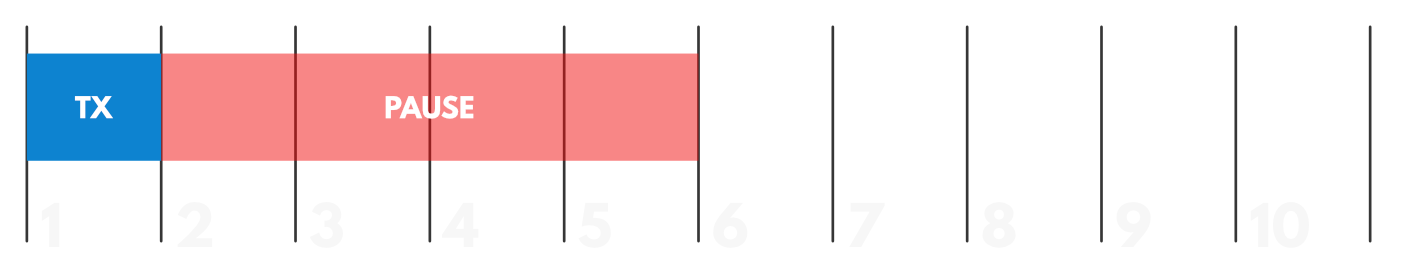
\includegraphics[width=.8\textwidth]{pictures/lora/duty-cycle-single-channel-off-air.png}
    \caption[Schematic example of duty cycle in \acs{LoRa}.]{
        Schematic example of duty cycle in \ac{LoRa}.
        For this example, the duty cycle is \SI{20}{\percent}.~\protect\cite{the_things_industries_bv_duty_nodate}
    }\label{pic:lora-duty-cycle}
\end{figure}

In the \ac{EU} region, the duty cycle for transmissions in the \SI{868}{\mega\hertz} band is limited to \SI{1}{\percent}~\cite[p. 29]{etsi_etsi_2012}.
This means that a \acl{LRED} using this frequency band may only transmit for \SI{1}{\percent} of a given time slot.
For example, if a \acl{ED} transmits data for \SI{1}{\milli\second}, it must stay silent for the following \SI{99}{\milli\second}.

An example for duty cycle time frames can be seen in \Cref{pic:lora-duty-cycle}.
In this example, the duty cycle is \SI{20}{\percent}.
The \acl{ED} that transmits for one block of time needs to stay silent for the next four time blocks before it can transmit again.
To stay compliant with the \SI{20}{\percent} duty cycle, it may start a new transmission starting with the sixth time block.

LoRa packets are typically small, consisting of only a few bytes, allowing for transmission in a short duration, typically in a matter of milliseconds.
Even when using \acs{SF}12, which is the slowest \acs{SF} available, the maximum packet size of \SI{51}{\byte} can be transmitted in  \SI{1232.9}{\milli\second}~\cite[p. 6]{the_things_network_lorawan_nodate}\cite[p. 10f]{lora_alliance_inc_lorawan_regional_2017}.
This makes it possible to transmit data up to every few minutes even with the largest possible packet size and still stay compliant with the duty cycle of \SI{1}{\percent}.

The ETSI standard also defines the \acf{ERP} that can be emitted from a \acl{ED}'s antenna in this frequency band as \SI{25}{\milli\watt}~\cite[p. 29]{etsi_etsi_2012}.
``\ac{ERP} is the power radiated from the tip of the antenna'' after taking into account the antenna's gain and the cable loss~\cite[p. 23]{faruque_radio_2015}.

\subsection{\acl{SF}: a trade-off between transmission time and interference resistance}\label{sec:spreading-factors}

The \ac{LoRa} modulation uses different \aclp{SF} to transmit data~\cite{the_things_network_spreading_2023}.
The \acl{SF} determines the \ac{CHIRP} rate and thereby the data rate and range of the transmission.

There are six different \aclp{SF} available in the \ac{EU} region, ranging from \ac{SF}7 to \ac{SF}12.
\ac{SF}7 offers the highest data rate and the lowest range, while \ac{SF}12 offers the lowest data rate and the highest range.

\begin{figure}[htbp]
    \centering
    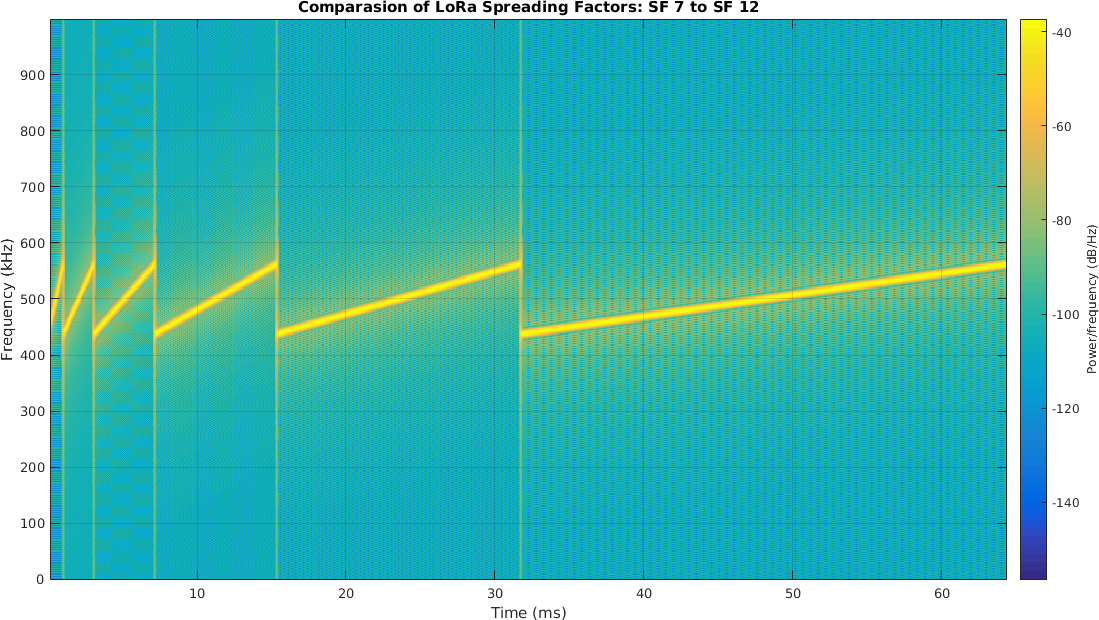
\includegraphics[width=0.7\textwidth]{pictures/lora/SF_Comparison_7_12.png}
    \caption[Comparison of \aclp{SF} 7 to 12 in the time and frequency dimensions.]{
        Comparison of \aclp{SF} \ac{SF}7 to \ac{SF}12 in the time and frequency dimensions.
        The doubling of the transmission time between increasing \aclp{SF} can be seen~\protect\cite{sakshama_ghoslya_lora_2017}.
    }\label{pic:lora-sf-comparison}
\end{figure}

\Cref{pic:lora-sf-comparison} shows the difference between different \aclp{SF} in the time and frequency dimensions.
It shows that the higher the \ac{SF}, the longer the transmission takes.
In fact, the transmission time is proportional to $2^{\text{SF}}$~\cite{sakshama_ghoslya_lora_2017}.
This means that, for example, a transmission using \ac{SF}10 takes twice as long as a transmission using \ac{SF}9.

While a higher \acl{SF} means that data can be transmitted over a longer range, the transmission also takes longer.
Given the 1\% duty cycle in the \ac{EU} region mentioned in \Cref{sec:duty-cycle}, this also means that using a higher \acl{SF} reduces the maximum amount of data that can be transmitted in any given timeframe.

Different \aclp{SF} are orthogonal to each other as far as \ac{RF} transmission through the air is concerned.
This means they can be used simultaneously without causing any interference with one another~\cite{the_things_network_spreading_2023}.

The \ac{SF} also determines the maximum size of the payload that can be transmitted.
In the \ac{EU} region, it ranges from \SI{222}{\byte} for \ac{SF}7 to \SI{51}{\byte} for \ac{SF}12~\cite[p. 10f]{lora_alliance_inc_lorawan_regional_2017}.

\subsubsection{Correlation of \acs{SF} and \acs{SNR}}\label{sec:sf-snr-correlation}

\aclp{SF} are important for this thesis because they interact with the \ac{SNR} values of a transmission.
Higher \ac{SF} values allow for lower \ac{SNR} values (more noise, less signal) to still be decodable, since the wider spread of the signal makes it more resilient to noise.

Because of this correlation between \acl{SF} and \acl{SNR}, it is essential to take both factors into account when performing similarity checks, such as fingerprinting as described in \Cref{sec:fingerprinting-additional-values}.

\subsection{Why use \acs{LoRa} over other technologies?}

As can be seen in \Cref{pic:wireless-protocols-comparison}, \ac{LoRa} is a good choice for \aclp{ED} that need to be able to operate battery-powered in remote locations for extended periods of time, as it has a long range and low power consumption.

A \ac{LoRa} \acl{ED} that transmits \SI{75}{\byte} of payload data every 2 hours can theoretically last up to 10 years on a single 1000 mAh battery~\cite{cheong_comparison_2017}.

LoRa Energy Calculator is a web application that can be used to roughly calculate the battery life of a \acl{LRED} by entering parameters such as payload size, data transmission periodicity and the battery type used~\cite{dramco_research_group_lora_2023}.
It calculates a ``worst case'' battery life of 6 years, 2 months and 1 week for a configuration with a payload size of \SI{8}{\byte}, 1 hour of periodicity and a 2500 mAh AA type battery.
The ``best case'' scenario is rated at 17 years, 4 months and 1 week.
Best and worst case scenarios use different \aclp{SF} and \ac{TP} and also consider when the message is acknowledged (RX1 or RX2 window, explained later in \Cref{sec:device-classes}).

\section{Connecting smaller networks to each other with \aclp{WAN}}

A \ac{WAN}, compared to a \acf{LAN} or \acf{MAN}, is a network that usually is not limited to one certain place, but connects multiple locations, across countries and continents~\cite[p. 2]{sadiku_fundamentals_2022}.
A well-known example of a \ac{WAN} is the Internet.

\begin{figure}[htbp]
    \centering
    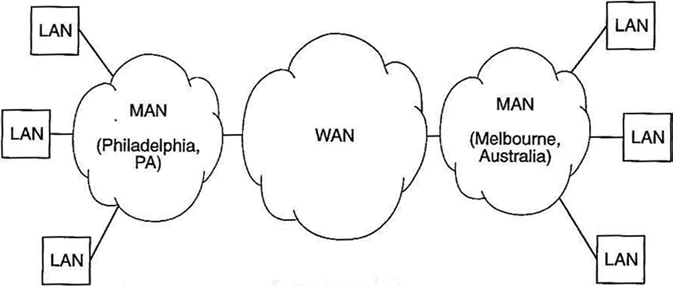
\includegraphics[width=.6\textwidth]{pictures/lorawan-structure/wan_diagram.png}
    \caption[An example connection between multiple \aclp{LAN} and \aclp{MAN}.]{
        An example connection between multiple \acp{LAN} and \acp{MAN} using a \acf{WAN} as a diagram~\protect\cite{sadiku_fundamentals_2022}.
    }\label{pic:wan-diagram}
\end{figure}

\Cref{pic:wan-diagram} shows the connections between \acp{LAN}, \acp{MAN} and \acp{WAN}.
\acp{WAN} consist of various \acp{MAN}.
\acp{MAN}, in turn, consist of various \acp{LAN}.

\subsection{Less power, longer latencies, low data rates — \aclp{LPWAN}}

While most \acp{WAN}, such as the Internet, typically have a high bandwidth and low latency, \acp{LPWAN}, on the other hand are designed to have ``low duty cycles, very low data rates, relatively longer latencies, low power consumption, and coverage over several kilometers''~\cite[p. 289]{kumar_connecting_2023}.
These factors make them more suitable for handling large amounts of \aclp{ED} that only need to transmit small amounts of data infrequently over long distances.

\begin{figure}[htbp]
    \centering
    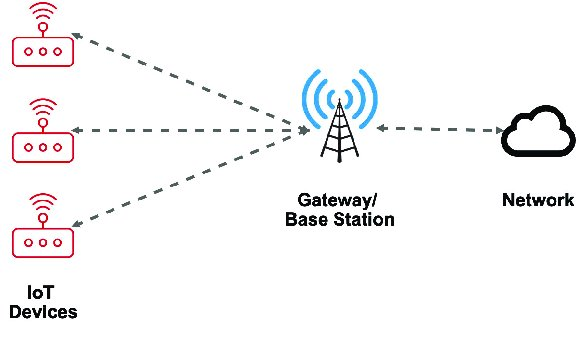
\includegraphics[width=.5\textwidth]{pictures/lorawan-structure/lpwan_network_structure.jpg}
    \caption[A diagram of \acl{LPWAN} network structure]{
        A diagram of \ac{LPWAN} network structure~\protect\cite{fernandez_assessing_2020}.
    }\label{pic:lpwan-diagram}
\end{figure}

\Cref{pic:lpwan-diagram} shows the structure of a \ac{LPWAN} network.
Multiple \ac{IoT} devices connect to \aclp{GW} or base stations.
Those \aclp{GW} are in turn connected to the network, enabling them to forward packets from \aclp{ED} to the network.

\section{\acl{LoRaWAN} — connecting \acl{IoT} devices over long ranges}\label{sec:lorawan}

\begin{figure}[htbp]
    \centering
    
\includegraphics[width=.3\textwidth]{pictures/logos/LoRaWAN_Logo.eps}
    \caption[\ac{LoRaWAN} logo]{
        \ac{LoRaWAN} logo~\protect\cite{lora_alliance_francais_2022}
    }
\end{figure}

\ac{LoRaWAN} uses the \ac{LoRa} wireless communication protocol to create a \ac{LPWAN} where multiple \aclp{LRWED} can communicate with each other over long distances.
It defines a secure way to transfer packets from the \acl{ED} to \acp{AS} by enforcing \ac{E2EE}.
This section will explain the structure of a \ac{LoRaWAN} network and how it works.

\subsection{\acs{LoRaWAN} network architecture — connecting \aclp{AS}, \aclp{GW} and \aclp{ED}}

\begin{figure}[htbp]
    \centering
    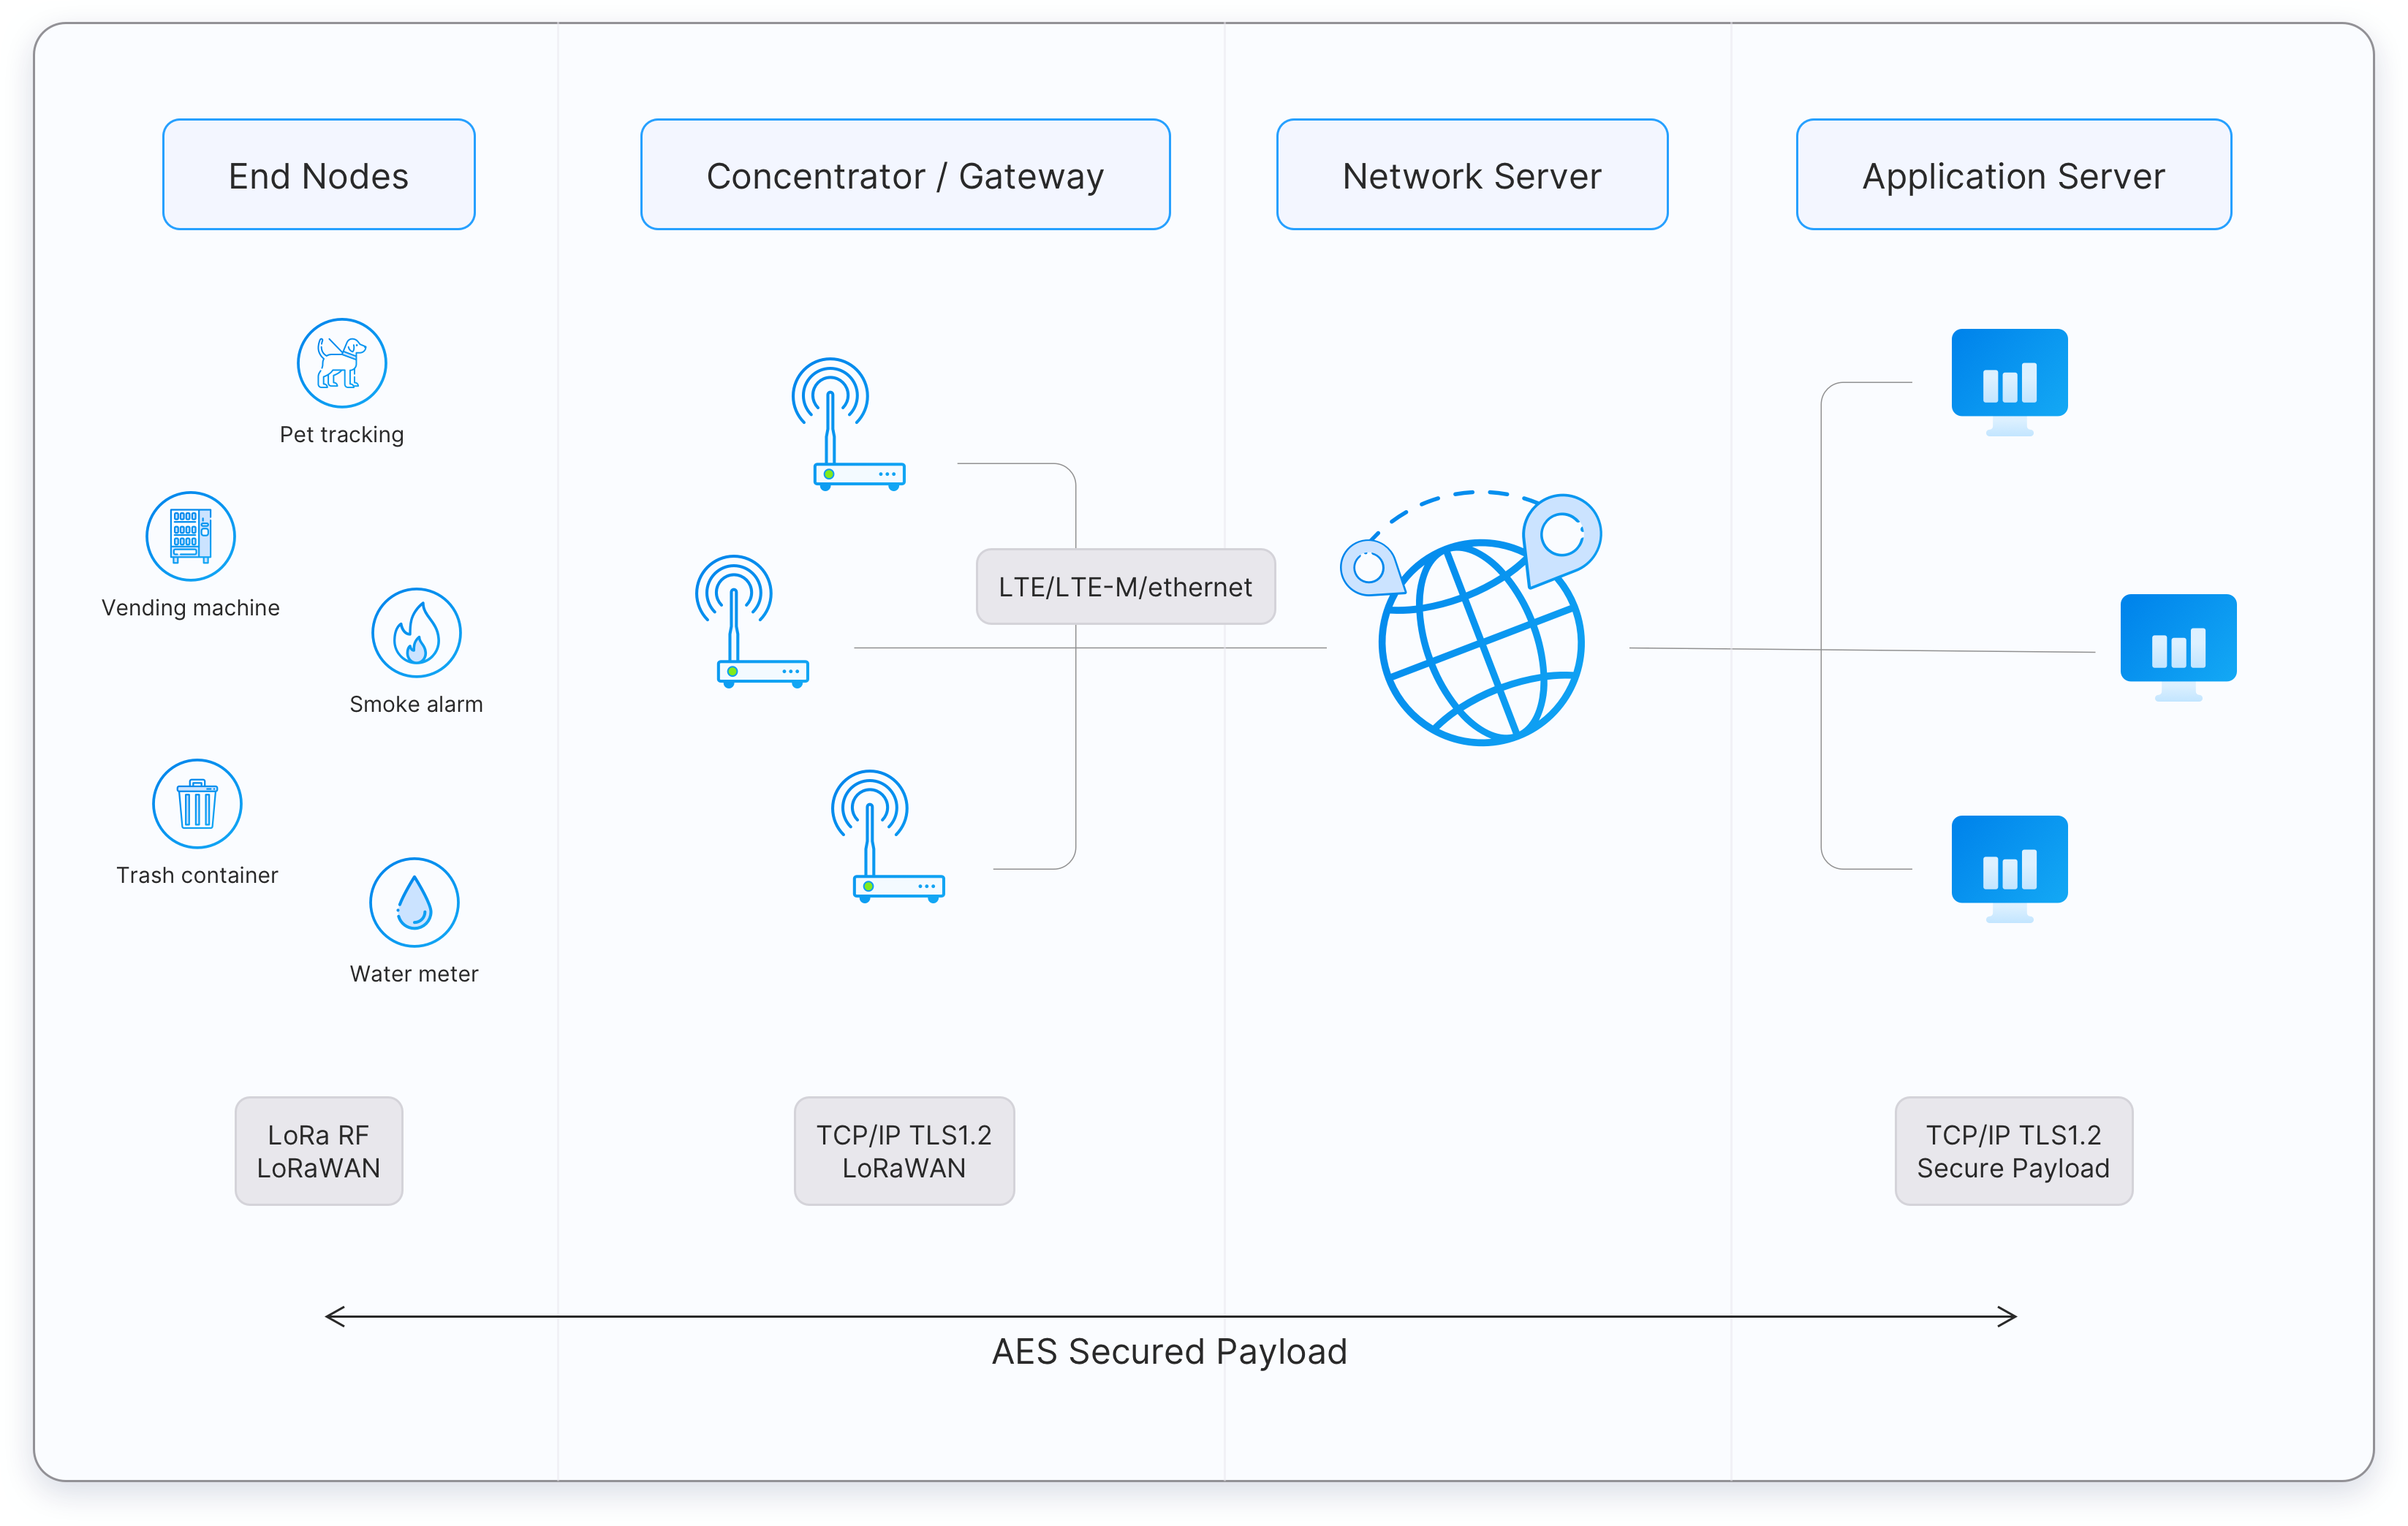
\includegraphics[width=1\textwidth]{pictures/lorawan-structure/lorawan-architecture.png}
    \caption[Structure of a \ac{LoRaWAN} network]{
        The structure of a \ac{LoRaWAN} network.~\protect\cite{the_things_industries_bv_lorawan_nodate}
    }\label{pic:lorawan-network-structure}
\end{figure}

The \ac{LoRaWAN} network architecture, as seen in \Cref{pic:lorawan-network-structure}, consists of four main components~\cite[p. 8]{lora_alliance_inc_lorawan_specification_2017}:

\begin{itemize}
    \item The end nodes (called \aclp{ED} in this thesis),
    \item the \aclp{GW} (also called concentrators or base stations),
    \item the \acf{LNS}, and
    \item the \acfp{AS}.
\end{itemize}

\ac{LoRaWAN} data rates typically range from 0.3 kbps to 50 kbps, depending on the region and the \ac{LoRa} modulation used~\cite[p. 8]{lora_alliance_inc_lorawan_specification_2017}.

\subsection{Connecting \aclp{ED} to the internet: \acs{LoRaWAN} Gateways}\label{sec:gateways}

\begin{figure}[htbp]
    \centering
    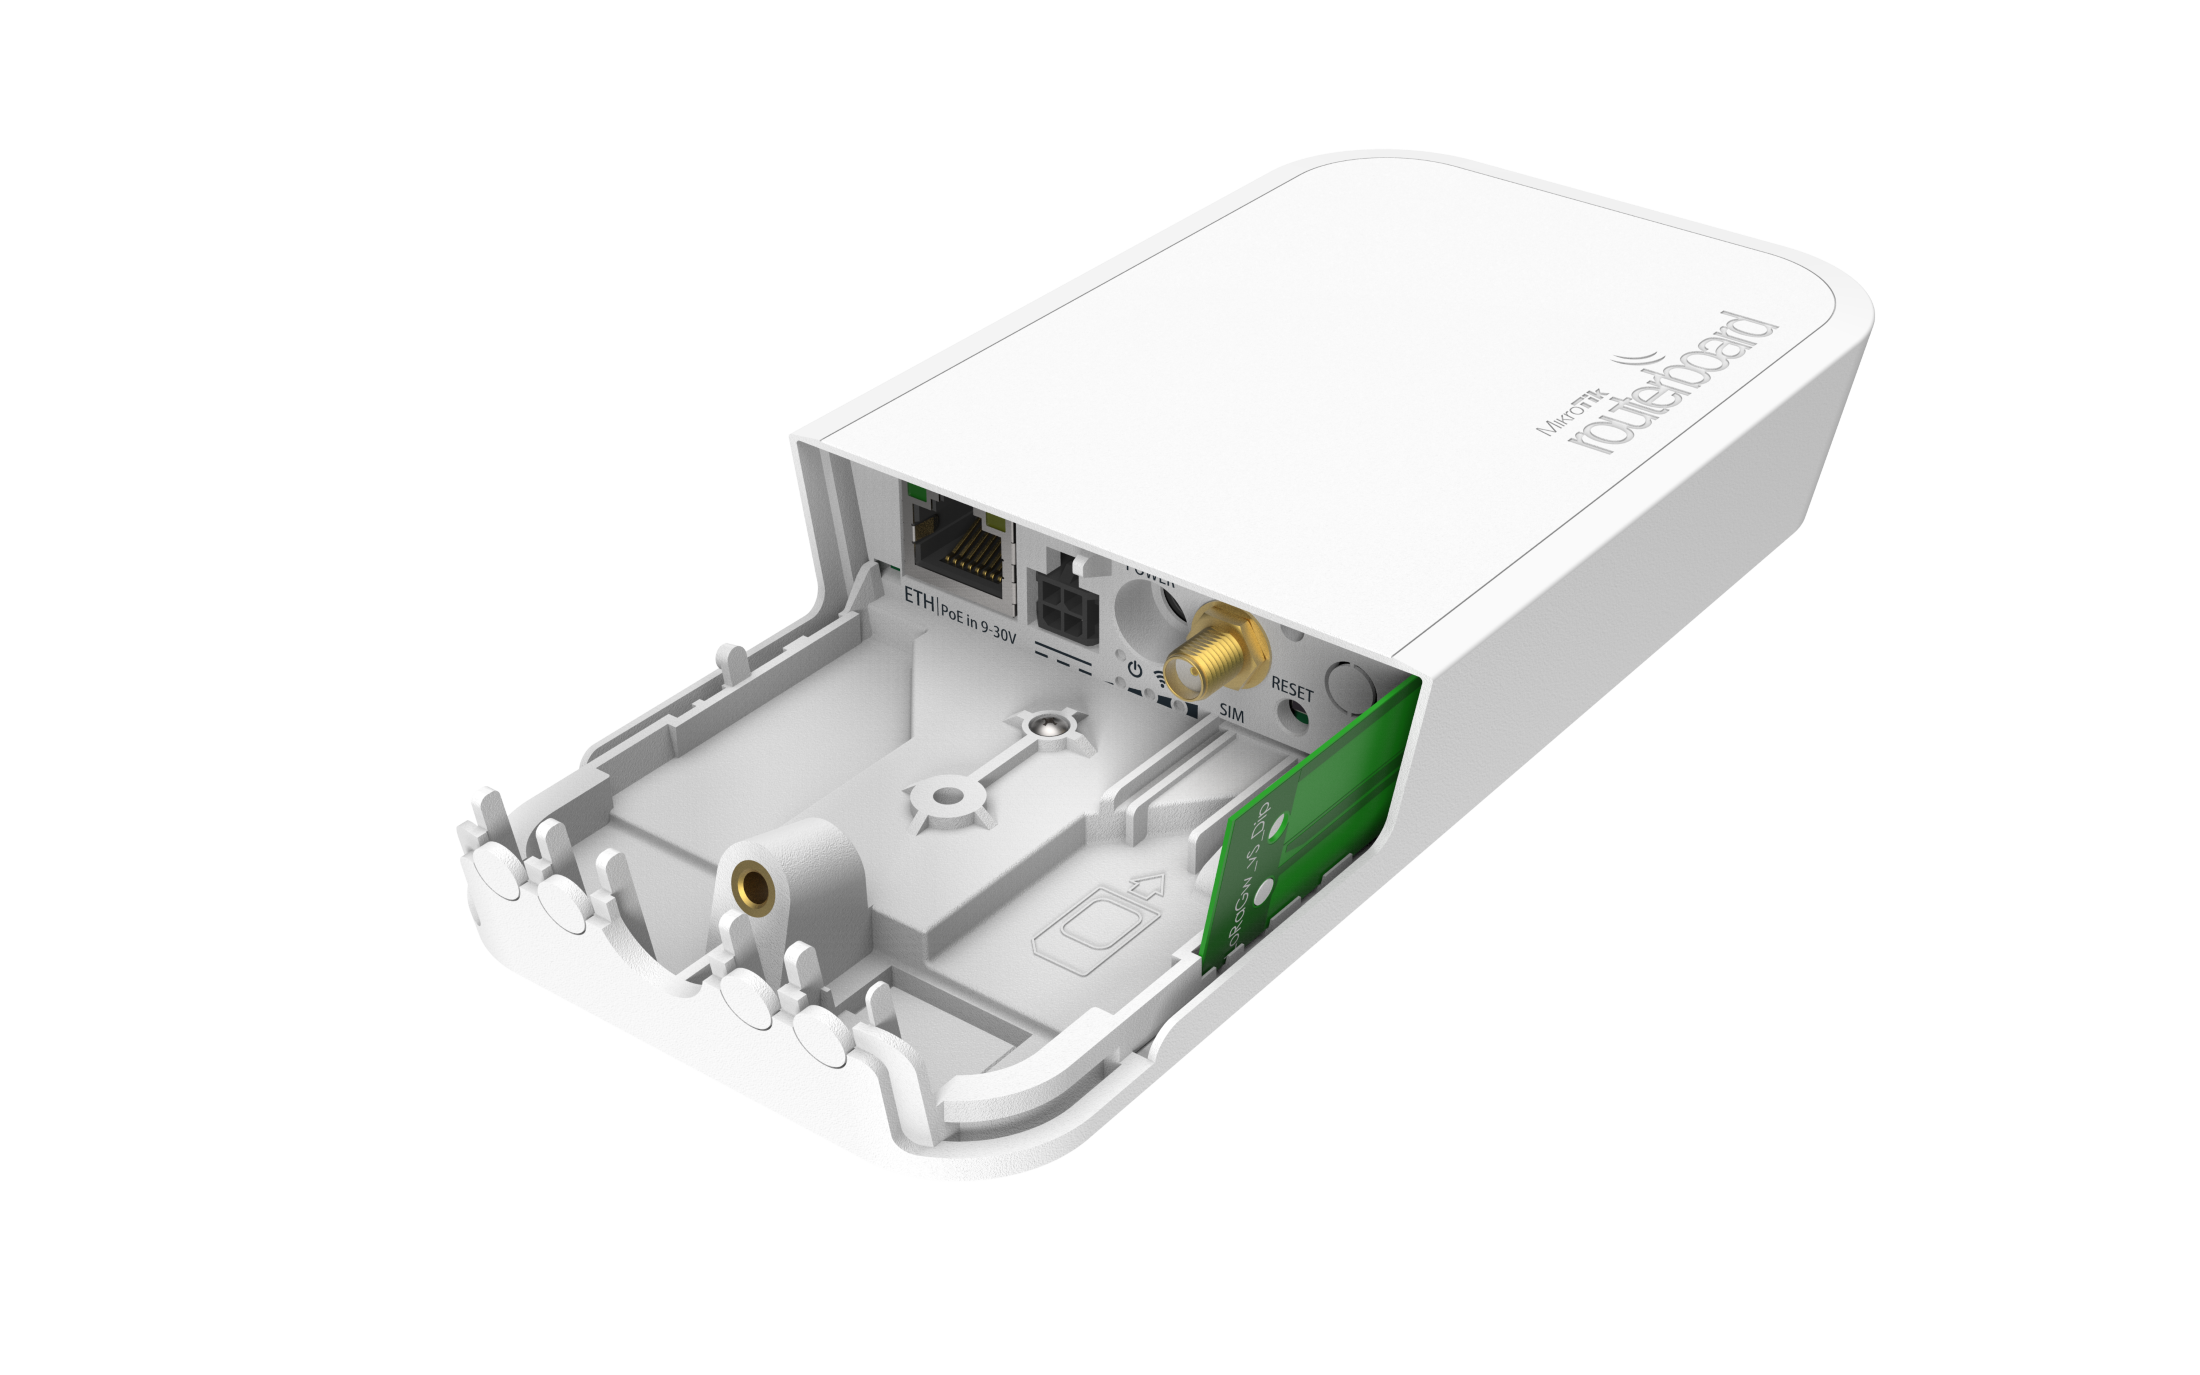
\includegraphics[width=.6\textwidth]{pictures/hardware/gateways/mikrotik-lr8-kit.png}
    \caption[Picture of a \acl{LRWGW}]{
        Picture of a \acl{LRWGW}, the MikroTik wAP LR8.
        This was one of the \aclp{LRWGW} used in this thesis.~\protect\cite{the_things_industries_bv_lorawan_nodate}
    }\label{pic:mikrotik-lr8-kit-gateway}
\end{figure}

A \acl{LRWGW} is a device that receives \ac{LoRa} packets (usually from \aclp{LRWED}) and forwards them to \ac{LNS}.
It can also receive packets from the \ac{LNS} and forward them to \aclp{LRWED}.

\aclp{LRGW} are usually based on a \ac{LoRa} concentrator, which is a \ac{RF} module that receives \ac{LoRa} packets and forwards them to the \acl{GW}'s \ac{CPU} using a serial interface.
The \ac{CPU} processes the incoming data and, if desired, forwards the packets to a \ac{LNS}.

To achieve the connection to the \ac{LNS}, the \acl{LRWGW} needs to be connected to the internet.
This connection is also called backhaul.
The most widely used methods to realize this are Ethernet/\ac{LAN}, Wi-Fi and \ac{LTE} connections~\cite{the_things_industries_bv_lorawan_nodate}.

One example of a \acl{GW} used during this thesis and therein installed in Furtwangen is the MikroTik wAP LR8 kit, as seen in \Cref{pic:mikrotik-lr8-kit-gateway}.

While some \aclp{LRWGW} may come equipped with an integrated antenna, their range is generally limited to small to medium-sized spaces or buildings.
It is also possible to use external antennas if it is necessary to cover a much larger area as was the case in this thesis since a medium to long range localization of \aclp{LRED} was the goal.

\subsection{Data Transmission between \aclp{LRWED} and \aclp{AS}}

In LoRaWAN, data transmissions from the \acl{ED} to the server and vice versa are called uplink and downlink, respectively~\cite[p. 12]{lora_alliance_inc_lorawan_specification_2017}.

Uplinks are relayed to the \ac{LNS} by one or more \aclp{LRWGW} from the \acl{LRWED}.
Downlinks, on the other hand, are only sent from the \ac{LNS} to the \acl{LRWED} using a single \acl{LRWGW}~\cite[p. 12]{lora_alliance_inc_lorawan_specification_2017}.

\subsection{Device Classes of \acs{LoRaWAN} \aclp{ED}}\label{sec:device-classes}

\ac{LoRaWAN} defines three device classes that offer different trade-offs between power consumption and availability~\cite[p. 10]{lora_alliance_inc_lorawan_specification_2017}.

\subsubsection{Lowest power communication: Class A}

\begin{figure}[htbp]
    \centering
    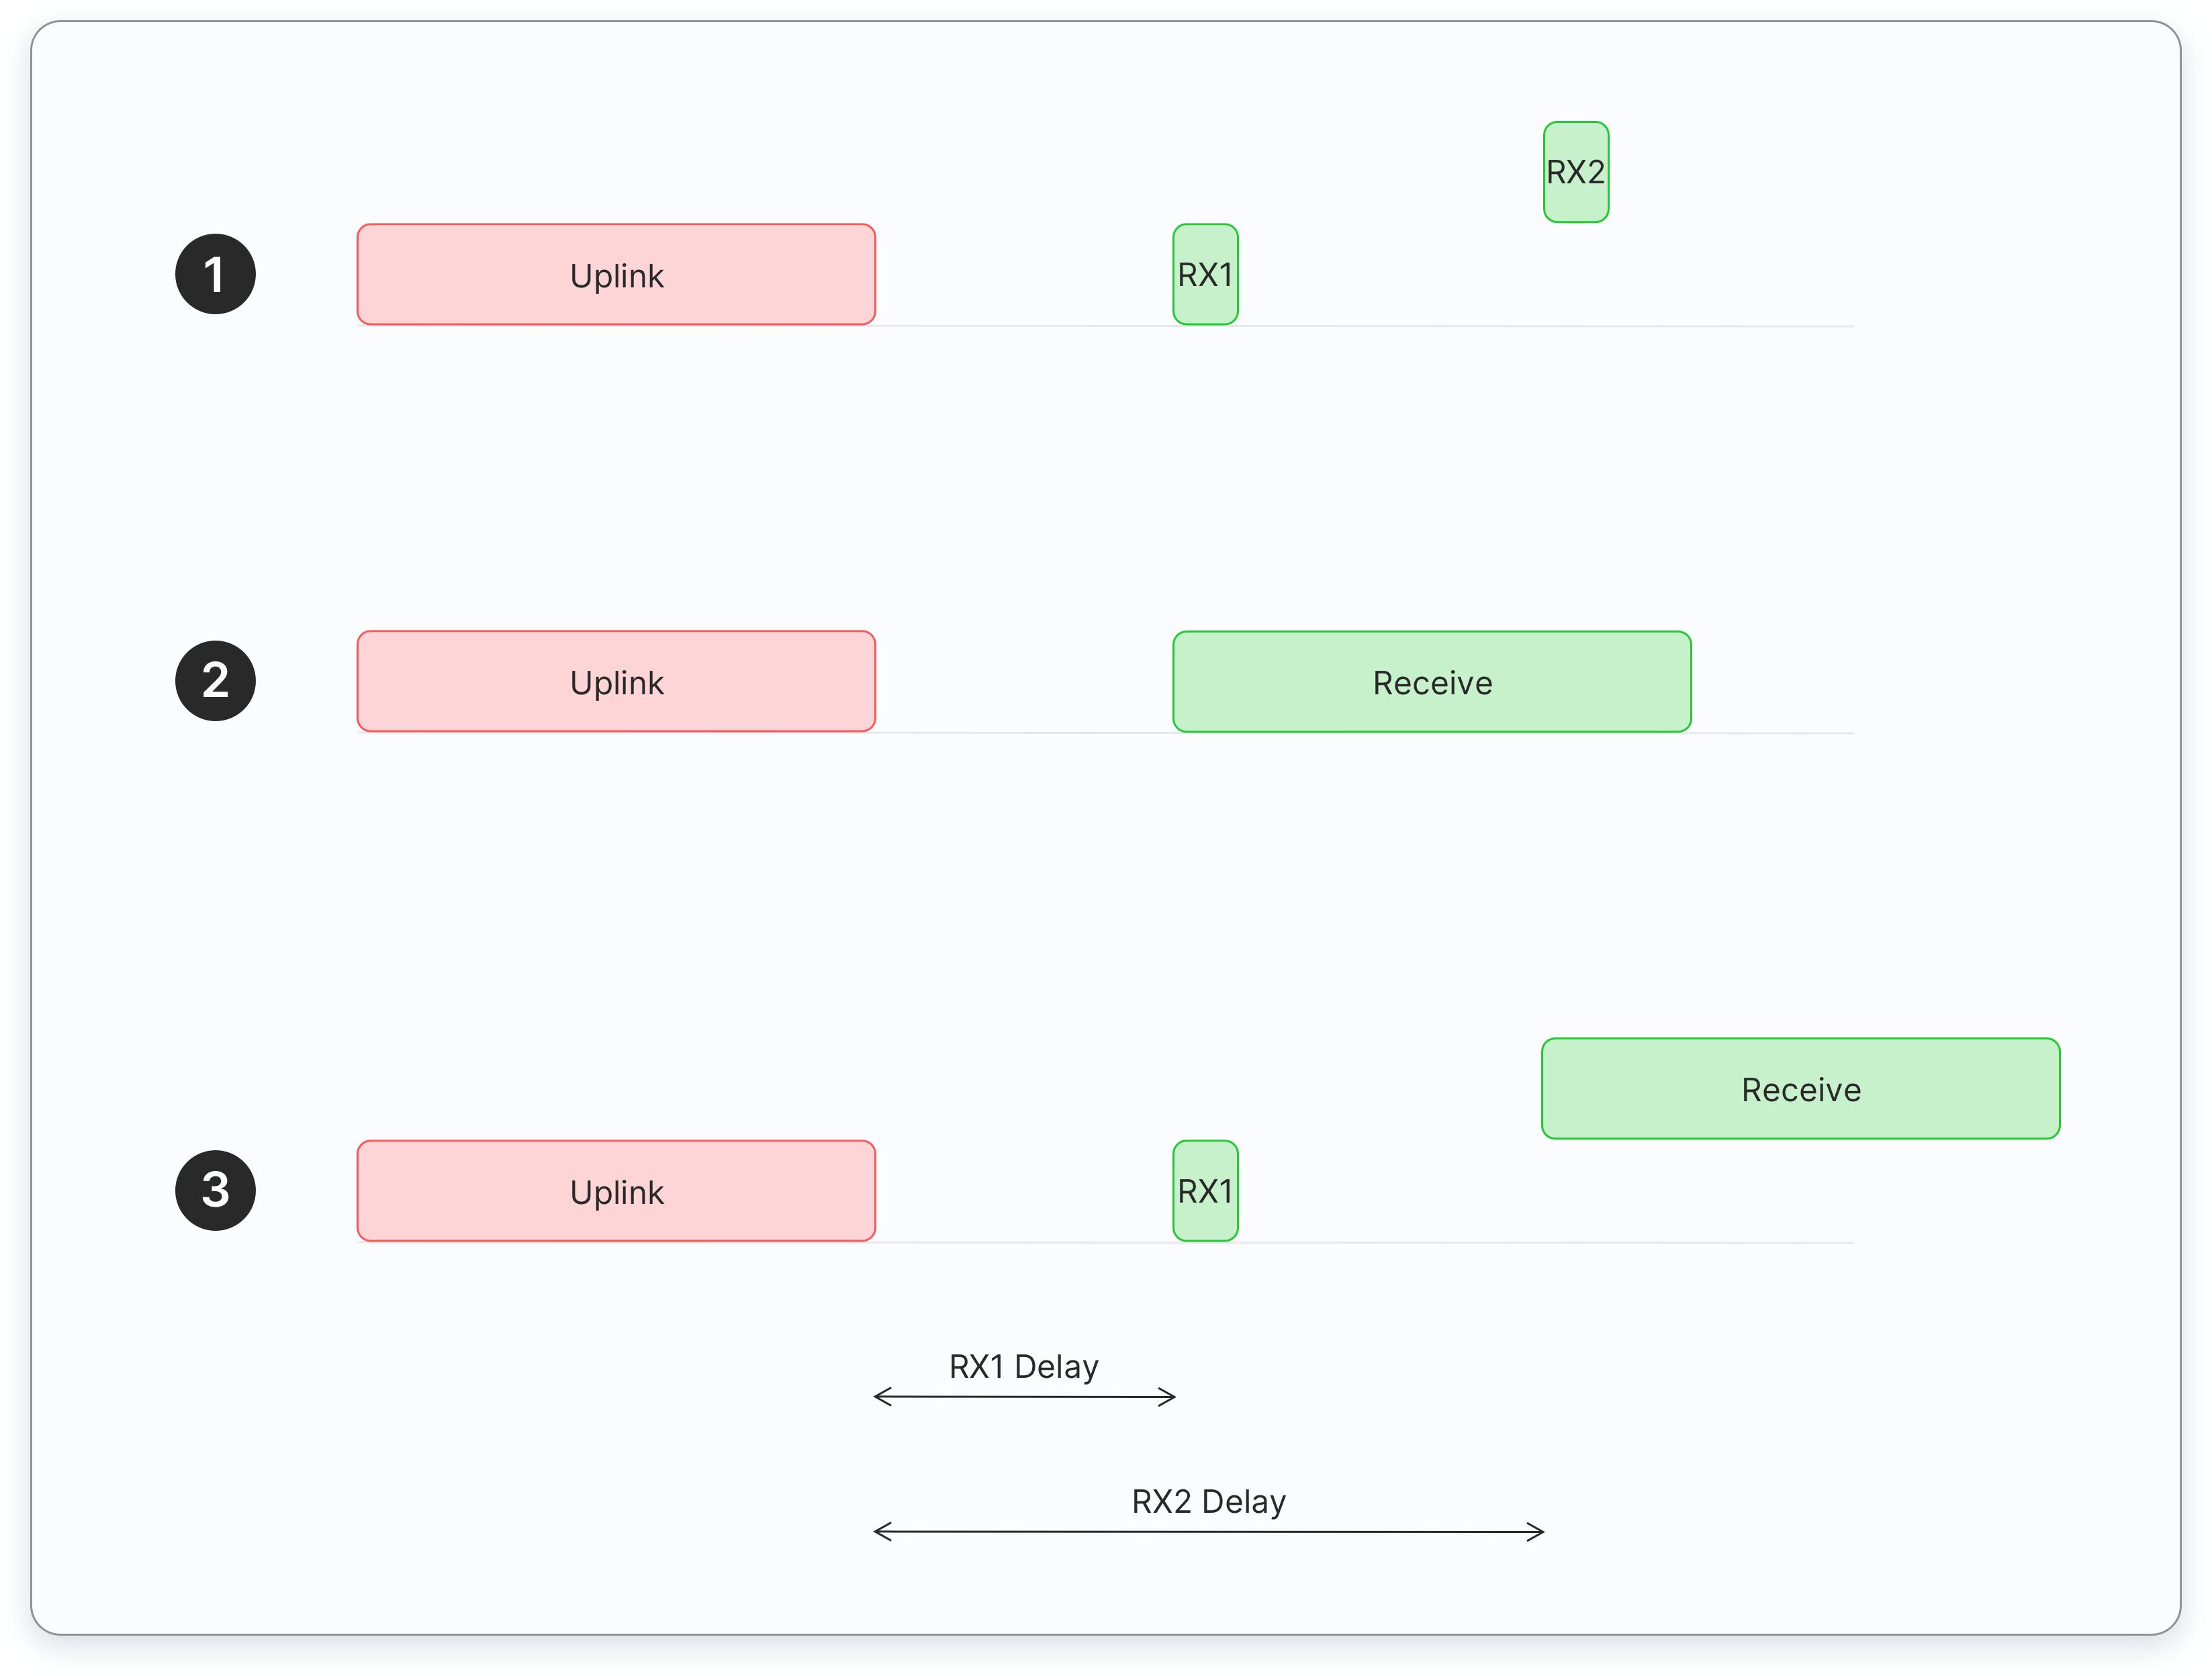
\includegraphics[width=0.9\textwidth]{pictures/device-classes/class-a.png}
    \caption[Schema of a \ac{LoRaWAN} Class A \acl{ED} communication]{
        A schema of a \ac{LoRaWAN} Class A \acl{ED} communication.
        The two receive windows (RX1 and RX2) are visible.~\protect\cite{the_things_industries_bv_device_nodate}
    }\label{pic:lorawan-device-class-a-schema}
\end{figure}

Class A is used for \aclp{LRWED} that need to consume as little power as possible.
Every \acl{LRWED} must support at least the Class A mode~\cite[p. 11]{lora_alliance_inc_lorawan_specification_2017}.
A communication in Class A is always initiated by the \acl{LRWED} itself.

Bidirectional communication is possible in Class A by means of two downlink receive windows, during which the \ac{LNS} can transmit data to the \acl{ED}~\cite[p. 13]{lora_alliance_inc_lorawan_specification_2017}.
An example can be seen in \Cref{pic:lorawan-device-class-a-schema}.

Class A consumes the least amount of power of the three classes, because \aclp{LRWED} in this class specify when and how often they want to communicate with the \ac{LNS}.
However, this also makes it impossible for the \ac{LNS} to send data to the \acl{ED} at any other time.

\subsubsection{Additional uplink windows: Class B}

\begin{figure}[htbp]
    \centering
    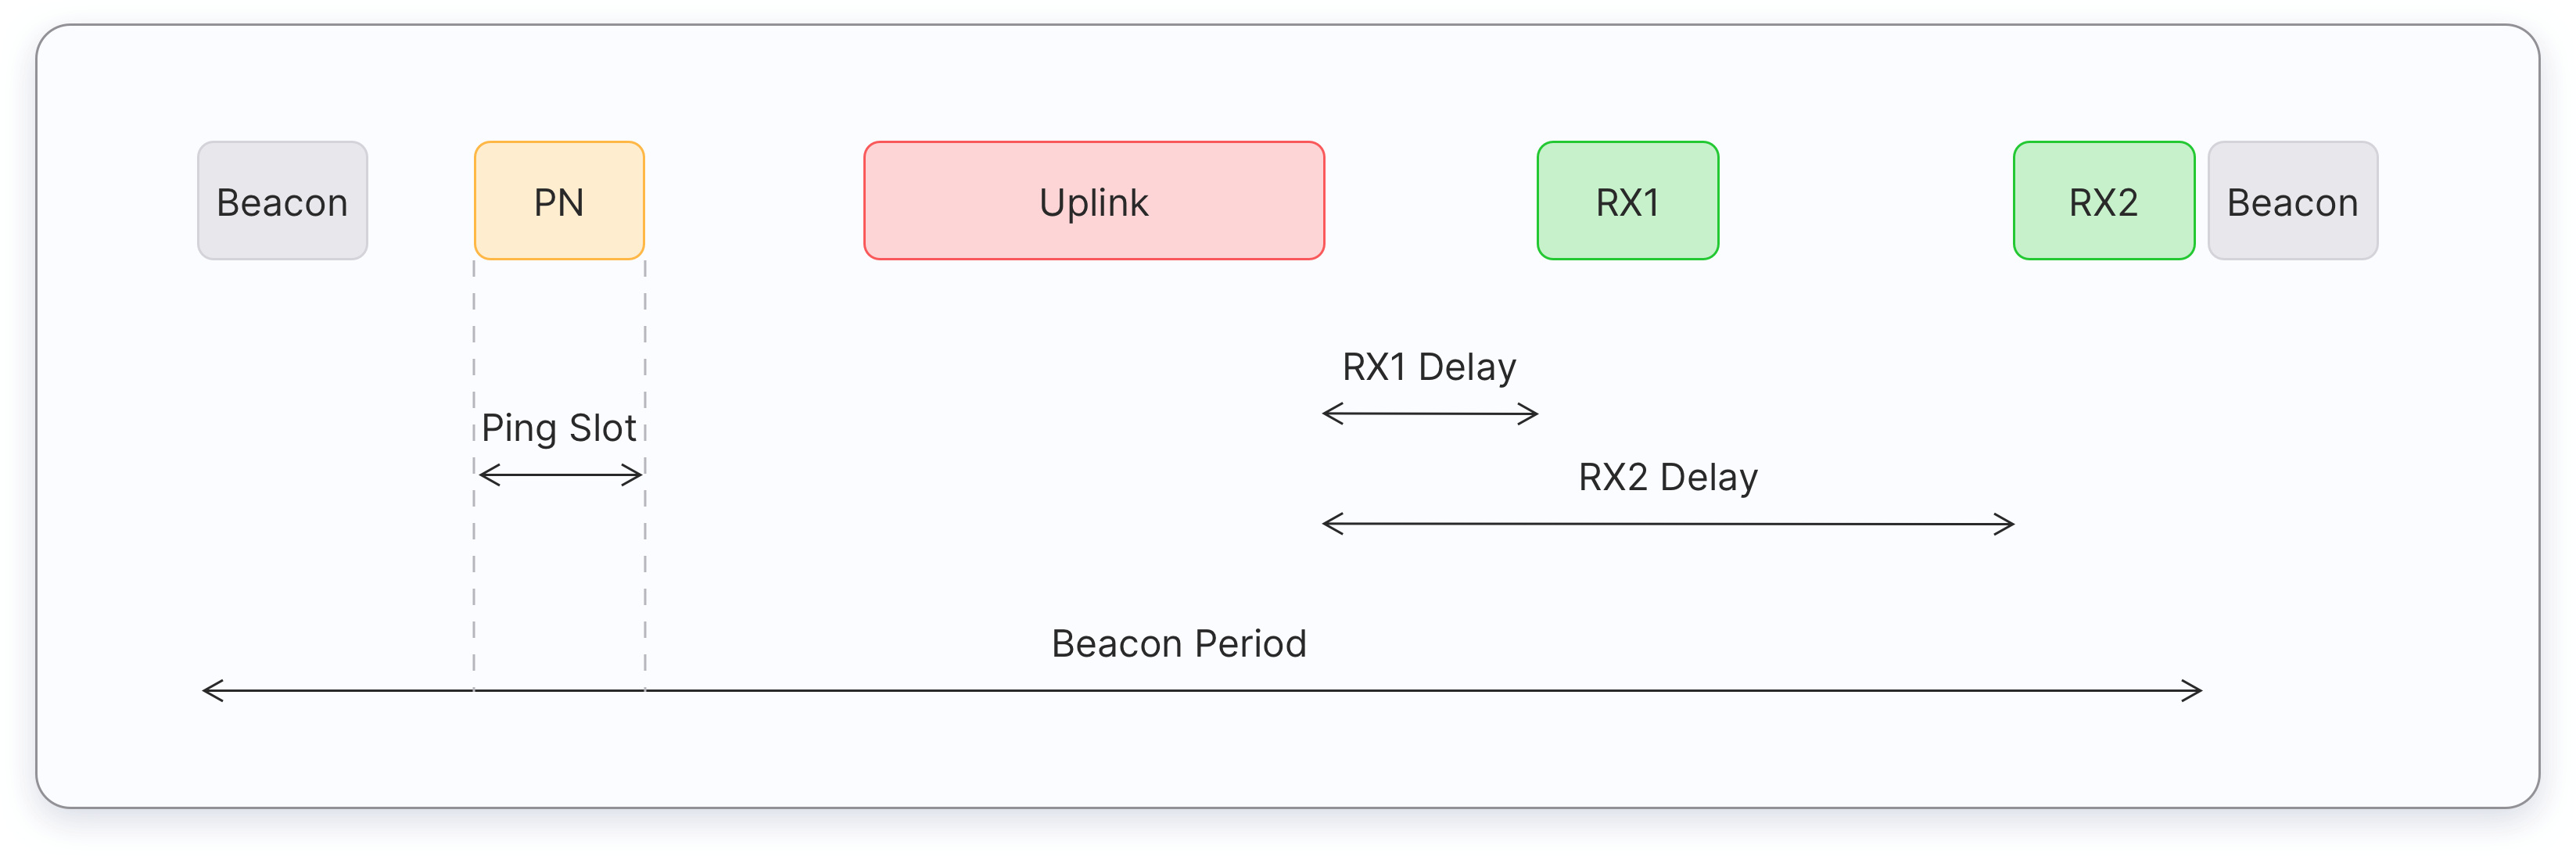
\includegraphics[width=0.9\textwidth]{pictures/device-classes/class-b.png}
    \caption[Schema of a \ac{LoRaWAN} Class B \acl{ED} communication]{
        A schema of a Class B \acl{LRWED} communication.
        The additional ping slots where the \acl{ED} is reachable by \aclp{LRWGW} can be seen.~\protect\cite{the_things_industries_bv_device_nodate}
    }\label{pic:lorawan-device-class-b-schema}
\end{figure}

In addition to the functionality provided by Class A, Class B \aclp{LRWED} are also able to receive downlink messages from the \ac{LNS} during dedicated downlink receive windows~\cite[p. 67]{lora_alliance_inc_lorawan_specification_2017}.
In order to realize this without the need for a per-device \ac{RTC}, such \aclp{ED} receive time synchronized beacons from the \aclp{LRWGW}.
The communication schema for Class B \aclp{LRWED} can be seen in \Cref{pic:lorawan-device-class-b-schema}.

These scheduled downlink windows result in a higher power consumption for Class B \aclp{LRWED}, because they need to be awake during these periods.

\subsubsection{Listening continuously: Class C}

\begin{figure}[htbp]
    \centering
    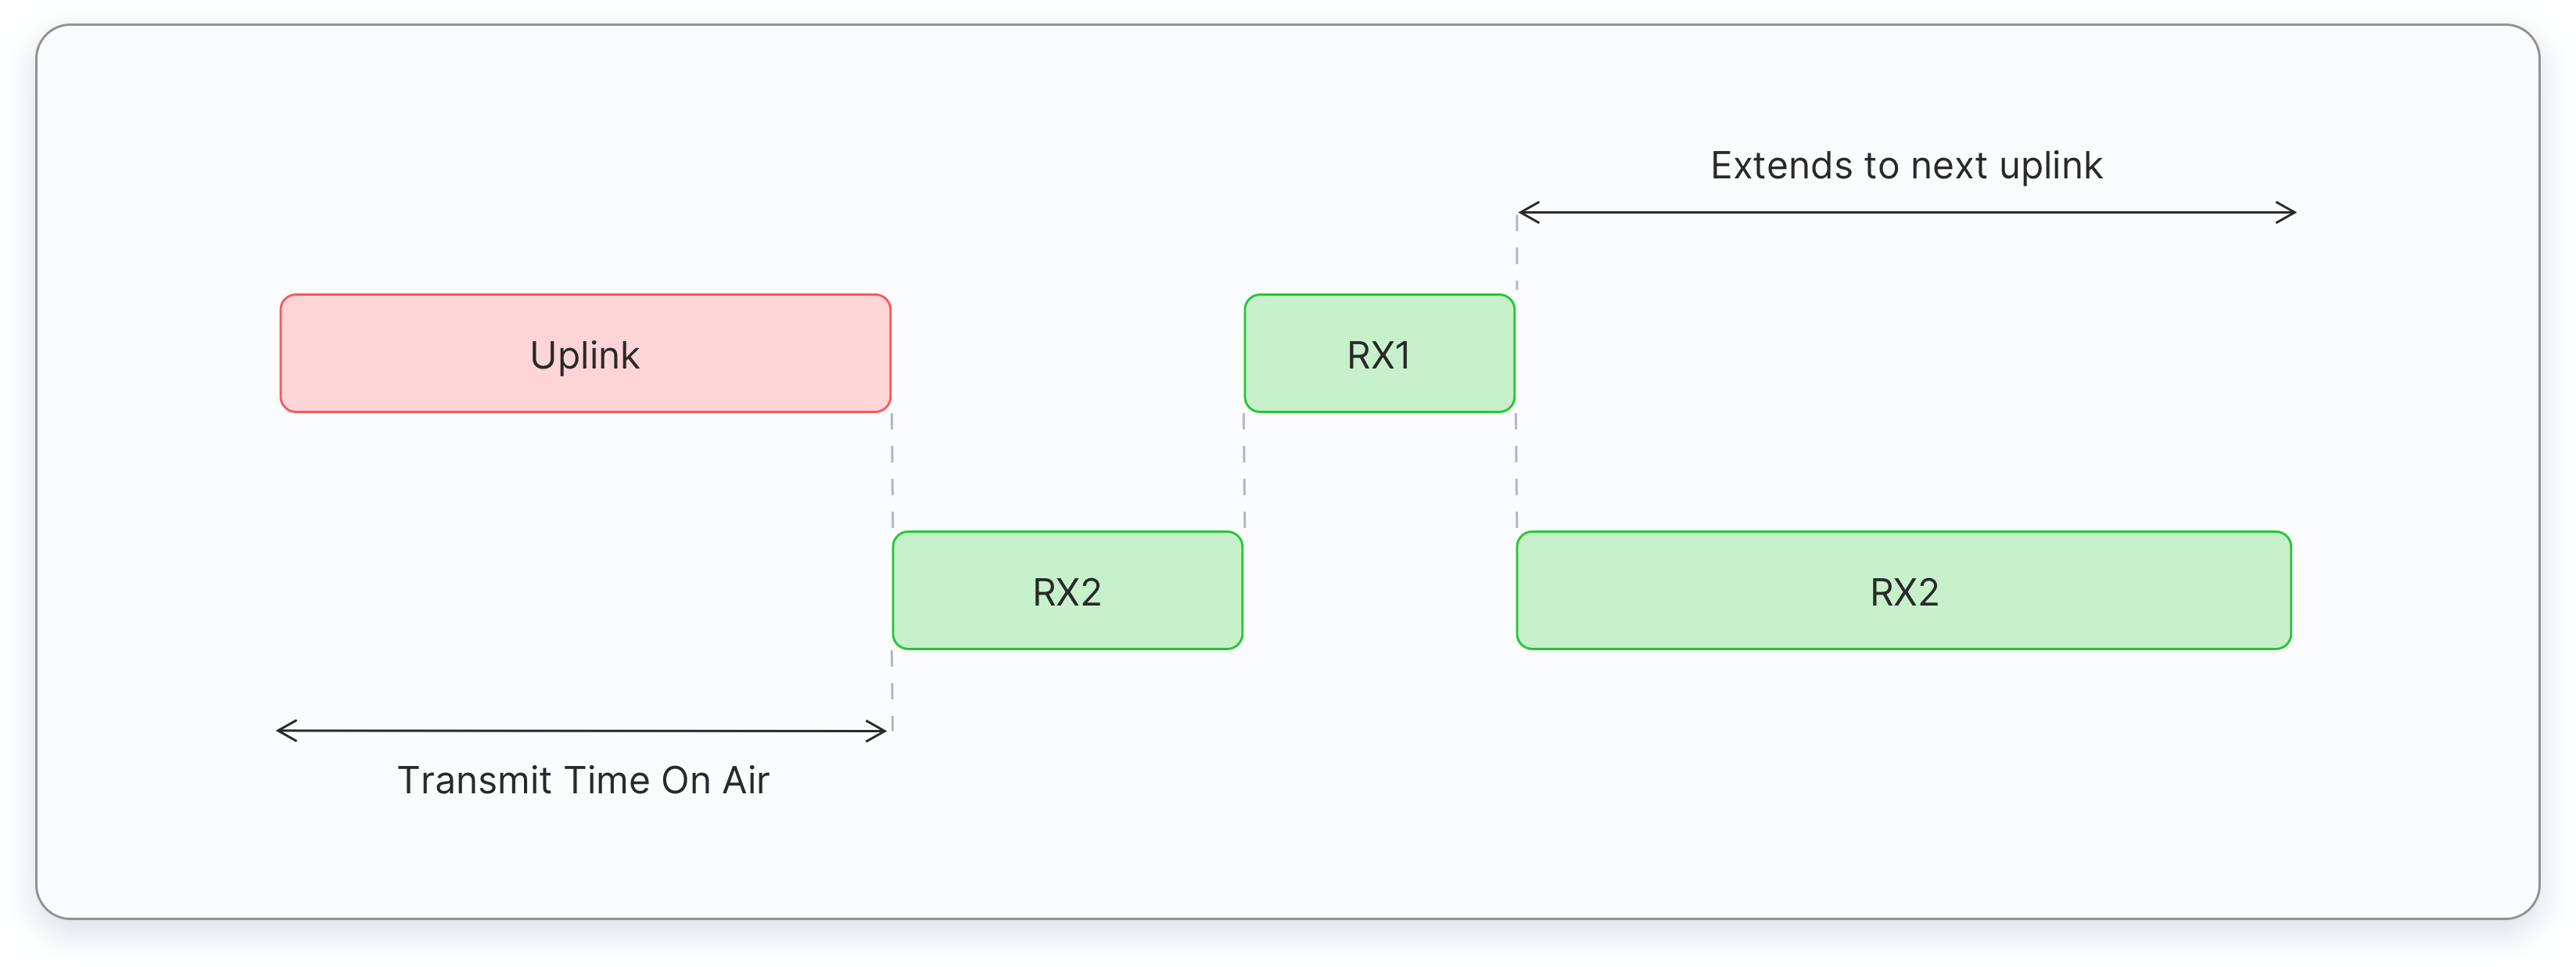
\includegraphics[width=0.9\textwidth]{pictures/device-classes/class-c.png}
    \caption[Schema of a \ac{LoRaWAN} Class C \acl{ED} communication]{
        A schema of a \ac{LoRaWAN} Class C \acl{ED} communication.
        The RX2 window is kept open between uplink transmissions to allow \aclp{LRWGW} to reach the \acl{ED} at any time while no uplinks are occurring.~\protect\cite{the_things_industries_bv_device_nodate}
    }\label{pic:lorawan-device-class-c-schema}
\end{figure}

Class C \aclp{LRWED} are always listening for downlink messages from the \ac{LNS} when not currently transmitting an uplink message~\cite[p. 86]{lora_alliance_inc_lorawan_specification_2017}.
In essence, they keep the downlink windows as specified in Class B open all the time as seen in \Cref{pic:lorawan-device-class-c-schema}.

As a result, \aclp{LRWED} in Class C consume the most power because they are always listening for downlink messages.
The fact that they are always reachable by the \ac{LNS} also makes them the most suitable for applications that require a high data rate or reliable downlink accessibility.

\subsubsection{Conclusion: Which device class was used?}

As far as this thesis was concerned, only Class A was used.
Class B and C use significantly more power than Class A because they keep their radio on for extended periods of time, which drains power quickly for battery-powered \aclp{ED}.

In their paper ``Comparison of LoRaWAN Classes and their Power Consumption'', Cheong et al.\ show that a \acl{LRWED} in Class C would need a battery approximately 19 times larger than a Class A \ac{ED} to achieve the same battery life with a packet size of 115 bytes and a transmission interval of 1 hour~\cite{cheong_comparison_2017}.
As mobile \aclp{LRWED} that need to be located are usually battery-powered, Class A is the most viable option for them.

The geolocation methods assessed in this thesis function with any \acl{LRWED} Class.
Although opting for Class C would enable direct location inquiries from the \aclp{LRWED} at any given time, selecting Class A is usually the preferred option due to its lower power consumption.

\subsection{Data security in \acs{LoRaWAN} transmissions}

The security of the data sent is a major concern when talking about \ac{IoT} protocols.
\ac{LoRaWAN} uses \ac{AES} based \acf{E2EE}.
Each \acl{ED} usually has a unique 128-bit \ac{AES} key that is used to encrypt the payload~\cite[p. 24]{lora_alliance_inc_lorawan_specification_2017}.

This \ac{E2EE} also makes \ac{LoRaWAN} packets secure against replay attacks (where a malicious attacker captures sent packets and sends them again), since a so-called \ac{MIC} is determined from the frame data.
This \ac{MIC} contains numbers that are incremented with each packet sent and are also encrypted along with the payload~\cite[p. 22f.]{lora_alliance_inc_lorawan_specification_2017}.

\section{\acl{TTN}: A community-based \acs{LoRaWAN} \acl{AS}}

\ac{TTN} provides a free to use \ac{SaaS} \ac{LNS} that has a global community of people building \ac{LoRaWAN} applications.
Its source code is also available on GitHub under the Apache 2.0 license~\cite{the_things_network_thethingsnetworklorawan-stack_2023}.

\begin{figure}[htbp]
    \centering
    
\includegraphics[width=0.2\textwidth]{pictures/logos/TTN-logo.eps}
    \caption[\acl{TTN} logo]{\acf{TTN} logo~\protect\cite{the_things_industries_bv_quick_nodate}}
\end{figure}


While it is officially called \acl{TTS Community Edition} since 2021, it is still commonly referred to as \acf{TTN} by the community itself~\cite{the_things_industries_bv_what_2022}.
Its users provide \ac{TTN} with \aclp{LRWGW} that other users can use, making it a crowdsourced \ac{LoRaWAN} network.

\subsection{Receiving packets from \aclp{LRWGW}}

\aclp{LRWGW} can forward \ac{LoRaWAN} packets that they receive to the \ac{LNS} in two commonly used ways.
This section will explain both of them.

\subsubsection{The older, simple way: \acl{SUPF}}

The \ac{SUPF} is a piece of software used to connect \aclp{LRGW} to the \ac{LNS}~\cite{the_things_industries_bv_semtech_2022}.
The \ac{SUPF} forwards \ac{LoRaWAN} packets that it receives from its connected \ac{LoRa} concentrator to the \ac{LNS} using the \ac{UDP} protocol.

\ac{TTN} marked the \acl{SUPF} as deprecated, since it ``has many security and scalability drawbacks``.
It is recommended to use the \ac{LBS} protocol instead~\cite{the_things_industries_bv_semtech_2022}.

\subsubsection{The modern way: \acl{LBS}}\label{sec:lorawan-lbs}

Since \ac{TTN} v3, using the \ac{TCP}-based \acl{LBS} protocol is recommended over the \ac{SUPF} to connect \aclp{LRWGW} to \aclp{LNS}~\cite{the_things_industries_bv_semtech_2022}.

\begin{figure}[htbp]
    \centering
    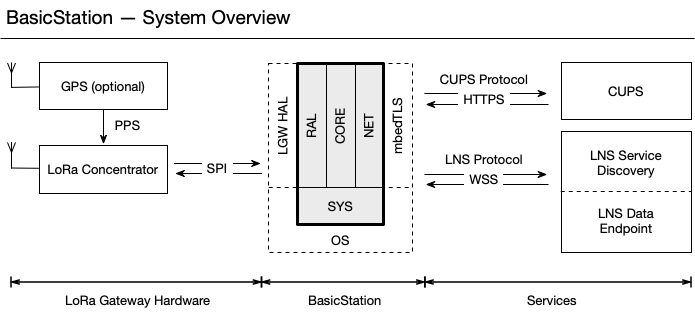
\includegraphics[width=1\textwidth]{pictures/lorawan-structure/lora-basics-station-structure.png}
    \caption[Schema of communications from a \acl{LRGW} and a \acl{LNS} using \acl{LBS}]{
        A schema of communications from a \acl{LRGW} and a \ac{LNS} using \acf{LBS}.
        The \ac{CUPS} service can be seen in the top right.~\protect\cite{semtech_lora_developer_portal_lora_2022}
    }\label{pic:lora-basics-station-schema}
\end{figure}

\ac{LBS} uses \ac{TLS}-encrypted \ac{TCP} connections with token-based authentication to relay \ac{LoRaWAN} packets to the \ac{LNS}~\cite{the_things_industries_bv_lora_2022}.

The two main components of \acl{LBS} are the \ac{LNS} connection itself as well as the \acf{CUPS}.
The communication schema can be seen in \Cref{pic:lora-basics-station-schema}.

The \ac{LNS} uses the \ac{WSS} protocol for communication and is responsible for handling the \ac{LoRaWAN} packets whereas the \ac{CUPS} is responsible for handling the configuration of \aclp{LRWGW}.

While \ac{CUPS} is not strictly necessary for actually sending \ac{LoRaWAN} packets, it simplifies the management of \aclp{LRWGW} and their configuration.
It communicates using \ac{TLS}-encrypted \ac{TCP} (\ac{HTTPS}) connections with token-based authentication.
When a \acl{LRWGW} is configured with \ac{CUPS}, it automatically receives its configuration from the \ac{LNS}.
As opposed to \ac{SUPF}, \ac{CUPS} also allows for remote configuration of \aclp{LRWGW} as well as remote firmware updates~\cite{the_things_industries_bv_lora_2022}.

\subsubsection{Conclusion: Which one was used?}

Some \aclp{LRWGW} used in this thesis were unable to use the more modern \acl{LBS} protocol.
This was the case for the MikroTik LR8 wAP \acl{LRWGW}, whose \ac{OS} RouterOS hadn't been updated to enable using \ac{LBS} at the time of writing this thesis.
It instead uses the \ac{SUPF} to forward \ac{LoRaWAN} packets to the \ac{LNS}.

Most of the other \aclp{LRWGW} deployed during this thesis, especially the ones from Dragino, were able to use \ac{LBS} and used it to forward \ac{LoRaWAN} packets to the \ac{LNS} in a more secure way as explained in \Cref{sec:lorawan-lbs}.

\subsection{\acl{TTN} Console — End Device and Gateway Management}\label{sec:web-interface-and-device-gateway-management}

\ac{TTN} provides a web interface for managing \aclp{LRWED} and \aclp{LRWGW} that are registered to the network by the logged-in user.
It also provides a \ac{REST} \ac{API} for managing \aclp{LRWED} and \aclp{LRWGW} programmatically.

\aclp{LRWED} are grouped into applications that can be used to manage \aclp{LRWED} that belong to a bigger project or \acl{ED} group.

In this thesis, an application was used to group the \ac{LoRaWAN} \ac{GPS} trackers that were used for data collection.

\subsection{Forwarding data from \acl{TTN} to \aclp{AS}}\label{sec:forwarding-data-from-ttn-to-as}

To transmit data from \ac{TTN} to an \ac{AS}, \ac{TTN} provides integrations~\cite{the_things_network_integrations_2021}.
\ac{TTN} offers several integrations for different cloud \acp{AS} such as \ac{AWS} \ac{IoT} Core and Microsoft Azure \ac{IoT} Hub.
It also provides a generic \ac{HTTP} webhook integration that can be used to forward data to any \ac{HTTP} or \ac{HTTPS} endpoint.

Additionally, \ac{TTN} provides a MQTT integration, which can send data to an MQTT broker.
MQTT is a widely used, lightweight publish-subscribe messaging protocol that is often used in \ac{IoT} applications~\cite{mqtt_mqtt_2022}.
The MQTT protocol is not used in this thesis, so it will not be discussed further.

\ac{TTNM}, the service that was used to collect geolocation data from \aclp{LRWED} in this thesis, uses a webhook integration to collect data from \ac{TTN}.
This is explained in more detail in \Cref{sec:ttm-data-collection}.

Integrations are managed on a per-application basis.
This means that different integrations can be used for different applications.

\subsection{Alternatives to \acl{TTN}}

While anyone can use the public \ac{SaaS} version of \ac{TTN} for free, it is not the only \ac{LNS} available.
\ac{TTN} can also be self-hosted, for example with Docker, using the open source \ac{LNS} \textbf{The Things Stack}~\cite{the_things_network_host_2023}.

There are also several other \acp{LNS} that can be used to build a private \ac{LoRaWAN} network:

\textbf{LORIOT} has a public community instance that acts similar to the \ac{SaaS} version of \ac{TTN}, and it also offers a self-hosted version~\cite{loriot_ag_loriot_2023}.
It is, contrary to \ac{TTN}, not open source.

Another popular \ac{LNS} is \textbf{ChirpStack}, which is open source and can be self-hosted~\cite{chirpstack_chirpstack_2023}.
Contrary to \ac{TTN}, it does not provide a \ac{SaaS} version and also does not offer a public community instance.

\section{\acl{TTNM} — Plotting \acs{LoRaWAN} reception on a map}

\acf{TTNM} was created by engineer JP Meijers in 2015~\cite{linkedin_23_nodate}.
He first created it as a personal project to map the range of his own \acl{LRWGW}.
However, the project has since been expanded to map the coverage of all public \aclp{LRWGW} registered in the public \ac{TTN} network instance~\cite{the_things_network_jp_2018}.
At the time of writing, this includes over 11,000 \aclp{LRWGW}.
This number was taken from the response of a \ac{TTN} \ac{API} route that \ac{TTNM} uses to display \acl{LRWGW} data.

\subsection{Data collection in \acl{TTNM}}\label{sec:ttm-data-collection}

\acl{TTNM} works by having \aclp{LRWED} with \ac{GNSS} modules send their location to the \ac{TTN} network via uplink messages.
Alongside the location information, packets from those \aclp{LRWED} that are processed by \ac{TTN} also include information about which \aclp{LRWGW} received them.

Hence, \acl{TTNM} can use the information about which \aclp{LRWGW} received the message and the location information of the \ac{GNSS} modules of those \aclp{LRWED}.
This is done by means of a webhook integration that sends the data to an endpoint of the \acl{TTNM} \ac{API} whenever a \acl{LRWED} sends a packet to the \ac{TTN} network as has been explained in \Cref{sec:forwarding-data-from-ttn-to-as}.
With this data, it can build a map displaying the coverage of \aclp{LRWGW} in the \ac{TTN} network.

\subsection{\acl{TTNM} frontend data views}

\begin{figure}[htbp]
    \centering
    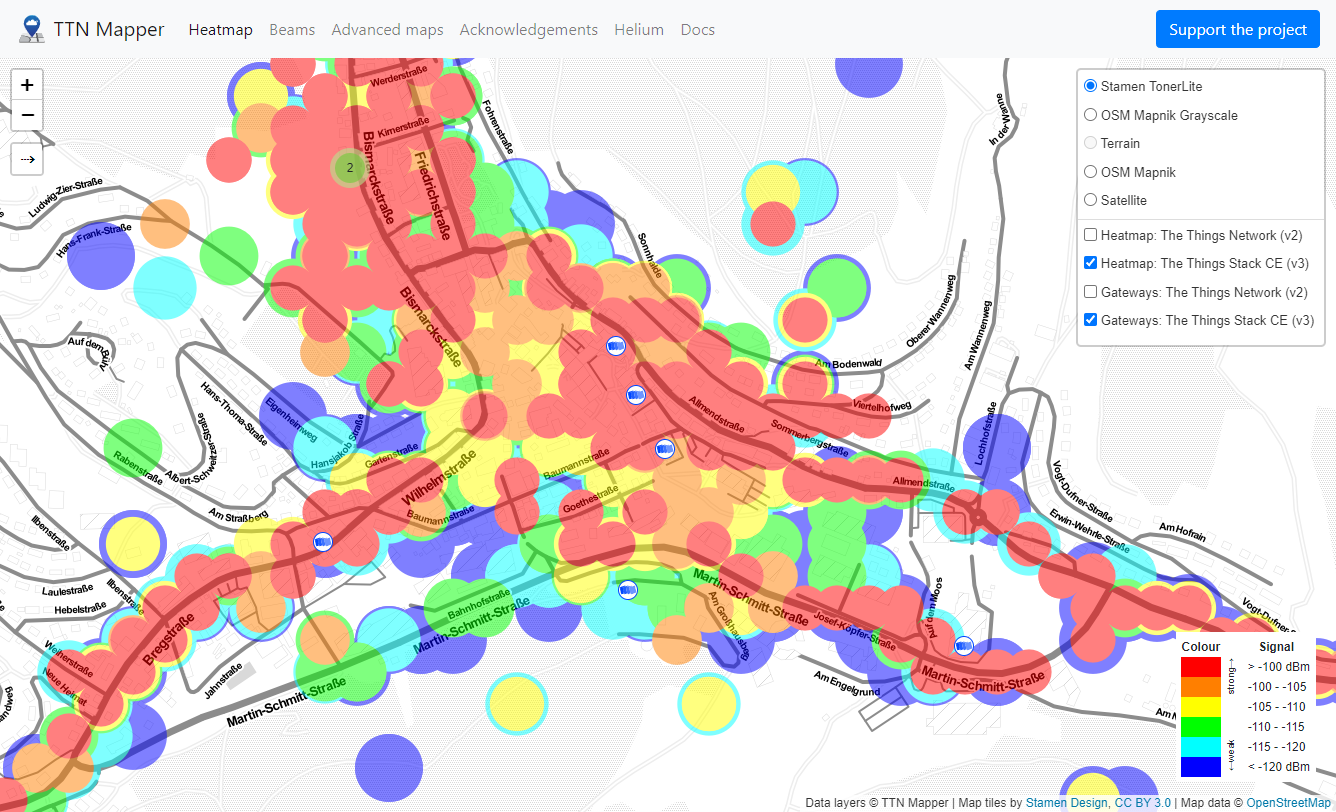
\includegraphics[width=0.9\textwidth]{pictures/ttn-mapper/heatmap_with_gateways.png}
    \caption[Screenshot of \acl{TTNM}'s heatmap view of the Furtwangen area.]{
        A screenshot of \ac{TTNM}'s heatmap view of the Furtwangen area.
        The heatmap shows places where strong signals where received by \aclp{LRWGW} in reddish colors.
        Weaker signals are shown in blueish colors.
        Some \aclp{LRWGW} are visible as small blue and white circles.
        This screenshot was taken at a time when considerable data collection had already taken place.
        \Cref{sec:collected-data-in-furtwangen-on-ttnm} will show before and after images of the same heatmap view for comparison.~\protect\cite{ttn_mapper_ttn_2023}
    }\label{pic:ttn-mapper-heatmap-with-gateways}
\end{figure}

\Cref{pic:ttn-mapper-heatmap-with-gateways} shows a screenshot of \acl{TTNM}'s heatmap view.
This page displays an interactive world map with a heatmap overlay.
It shows the coverage of \aclp{LRWGW} in the \ac{TTN} network by using and aggregating data that has been collected over the lifetime of the service.
Additionally, any \acl{LRWGW} that has received at least one message from a \ac{GNSS}-enabled \acl{LRWED} and has its location publicly accessible from \ac{TTN} is displayed on the map.

Notably, empty areas on the map do not necessarily indicate a lack of coverage in that region.
It simply implies that there have not been any \ac{GNSS}-enabled \aclp{LRWED} that have transmitted their data to \ac{TTNM} in that area yet.

\subsection{Accessing the data of \acl{TTNM}}

\ac{TTNM} provides a (partially) open \ac{REST} \ac{API} that can be used to access the data that has been collected by it.
Data can be requested based on the \acl{LRWED} that sent the message or based on the \acl{LRWGW} that received it.
In addition, the data can be filtered by the time that it was recorded on.
The data is provided in graphical (map-based) form as well as in \ac{CSV} files.

There is an additional non-documented part of the \ac{API} that can be used to access the data in \ac{JSON} form.
This was the part of the \ac{API} that was used most for this thesis.

\subsection{Importance of \acl{TTNM} for this thesis}\label{sec:ttn-mapper-importance}

The data that is provided via the \ac{TTNM} \ac{REST} \ac{API} served as the foundation of this thesis.
The \ac{TTNL} application that will be described in \Cref{section:ttnl} was created to access this \ac{API} and request its data to make it possible to perform advanced queries on it.
Such queries were not possible with the \ac{TTNM} \ac{API} alone, since it doesn't provide direct access to its underlying \ac{DB} or provide specific endpoints for the kind of complex data filtering that was needed for this thesis.

Through building a \ac{DB} of \ac{RSSI} and location values, \ac{TTNM} also enables the use of the fingerprinting localization technique, as will be explained in \Cref{sec:rssi-fingerprinting}.
This was one of the techniques used to locate \aclp{LRWED} in this thesis.

\section{Multilateration — Locating devices using distances to reference points}\label{sec:multilateration-basics}

In everyday language, people often use the term triangulation or when talking about the process of determining the location of a \acl{ED} based on the distance to multiple other \aclp{ED}.
However, triangulation uses the angles between devices and three reference points to determine the location of the device, hence its name~\cite{yaro_multiangulation_2017}.
This process requires the \acl{ED} to be able to determine the angles to the reference points, which needs specific hardware.

\begin{figure}[htbp]
    \centering
    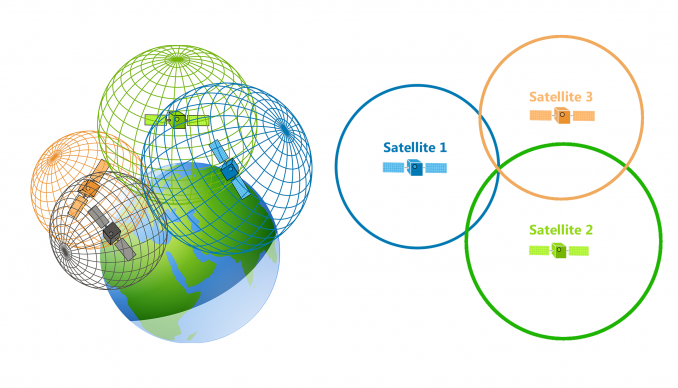
\includegraphics[width=0.8\textwidth]{pictures/multilateration/gps_multilateration.png}
    \caption[Example of how multilateration works in the \acl{GNSS} in 2D and 3D]{
        An example of how multilateration works in \ac{GNSS} in 2D and 3D~\protect\cite{gisgeography_how_2018}.
        It can be seen that 4 Satellites are needed to get a three-dimensional fix while only 3 are needed for a two-dimensional fix.
    }\label{pic:multilateration-gps-2d-3d-example}
\end{figure}

The correct term to use when using distances between an \acl{ED} and multiple receivers to achieve a localization of the \acl{ED} is multilateration.
An example of this in \ac{GNSS} is shown in \Cref{pic:multilateration-gps-2d-3d-example}.
A specific case of multilateration is trilateration, which specifies three receivers to get the ranges from~\cite{ruiz_efficient_2013}.

\section{Locating devices accurately outdoors with the \acl{GNSS}}

\ac{GNSS} is a generic term for systems that use satellites orbiting the Earth to determine the location of a \acl{ED}.
In everyday language, the term \ac{GPS} is often used as a synonym for \ac{GNSS}.
However, \ac{GPS} is only one of the several \ac{GNSS} systems that are currently in use.

\ac{GNSS} systems use multilateration to determine the location of \aclp{ED} as explained in \Cref{sec:multilateration-basics}.
\Cref{pic:multilateration-gps-2d-3d-example} shows an example of how this works with \ac{GNSS} satellites in 2D and 3D.

To determine the distance from the \acl{ED} to the satellites, the time it takes for a signal to travel from the satellite to the \acl{ED} is measured and used in conjunction with the speed of light to calculate the distance.
This approach is called \acf{ToA} and will be explained in more detail in \Cref{sec:toa-based-multilateration}.

\subsection{The most well-known \acl{GNSS} — The \acl{GPS}}

\ac{GPS} is the \ac{GNSS} system that is operated by the United States of America and is officially named NAVSTAR \ac{GPS}~\cite{department_of_defense_usa_gps_2020}.
The version of \ac{GPS} the public has access to is called \acf{SPS}.
Additionally, there is the \acf{PPS} that is only available to the military and other authorized users~\cite{department_of_defense_usa_gps_2007}.

Using an iPhone 6, Merry and Bettinger measured the accuracy of \ac{GPS} to be between 7 and 13 meters in an urban environment~\cite{merry_smartphone_2019}.

\subsection{Other established \aclp{GNSS}}

There are several other \ac{GNSS} systems in use or in development by different countries.
For example, the Russian GLONASS, the European Galileo, the Chinese \acf{BDS}, and the Indian \acf{IRNSS}.

Most modern smartphones support multiple \ac{GNSS} systems to enhance location accuracy.
One of Samsung's most recent devices as of writing this thesis, the Galaxy S23 Ultra, supports \ac{GPS}, GLONASS, Galileo, and \ac{BDS}, for example~\cite{gsmarena_samsung_2023}.

The \aclp{LRWED} used in this thesis, as described in \Cref{subsec:used-lora-devices}, only use \ac{GPS} to determine their location.

\subsection{A measure of \acl{GNSS} localization accuracy: \acl{HDOP}}

When talking about how accurate a certain data point of a \ac{GNSS} system is, the term \ac{HDOP} is used regularly.
There are multiple different terms that can be used to describe such accuracies: \ac{HDOP}, \ac{PDOP}, \ac{VDOP}, \ac{TDOP}, and \ac{GDOP}~\cite{langley_dilution_1999}.
As far as two-dimensional positioning is concerned, \ac{PDOP} and \ac{HDOP} are relevant.

\ac{PDOP} is calculated by using the position of satellites as well as the position of the \acl{ED}.
For example, ``on a 24-satellite constellation […], a 5-degree satellite elevation mask angle with no obstructions, and at least four satellites in view [results in a] \acf{PDOP} of six or lower''~\cite{langley_dilution_1999}.
Therefore, \ac{PDOP} is a measure of the quality of the current \ac{GNSS} constellation for a user.

\begin{figure}[htbp]
    \centering
    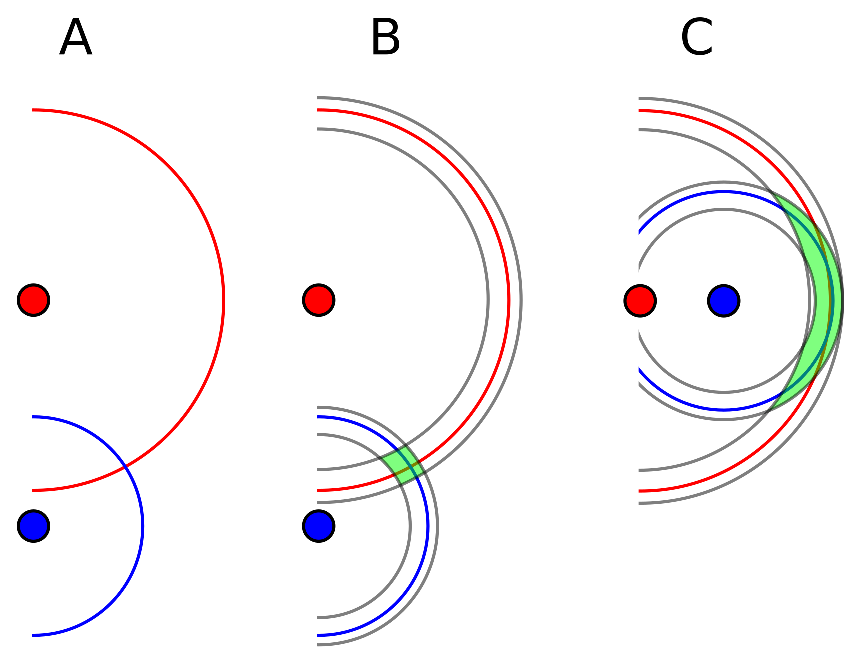
\includegraphics[width=0.5\textwidth]{pictures/multilateration/Geometric_Dilution_Of_Precision.eps}
    \caption[Examples for different kinds of \acl{HDOP} values]{
        Examples for different kinds of \ac{HDOP} values.
        A shows a (unrealistic) perfect example where there are no error margins --- a theoretical \ac{HDOP} of 0.
        B shows an example with error margins but a low \ac{HDOP}.
        The intersection area between the two annuli is small, therefore the error margin is small.
        C shows an example with a high \ac{HDOP}.
        The intersection area between the two annuli is large, therefore the error margin is large.\cite{xoneca_english_2013}
    }\label{pic:hdop-example-diagram}
\end{figure}

\ac{HDOP}, on the other hand, is a measure of the quality of a two-dimensional location fix.
\Cref{pic:hdop-example-diagram} shows three examples of different \ac{HDOP} scenarios.

The \ac{HDOP} value is relevant to this thesis because it was used to filter out values that were not considered accurate enough to be used in further calculations.
It is usually included in \ac{LoRaWAN} packets sent to \ac{TTN} from \ac{GPS} trackers.
As mentioned in \Cref{subsec:cleaning-collected-data}, \ac{TTNM} also excludes certain data points based on the \ac{HDOP} value.

\subsection{Power usage of localization via \acl{GPS} vs. \acs{LoRaWAN} metadata}\label{subsec:gnss-power-usage}

In order to demonstrate the significance of employing \ac{RSS} values rather than \ac{GNSS} systems for locating \aclp{ED}, this section provides a comparison of power usage between the two methods.

The ELV-LW-GPS1 module is a \ac{GPS} tracker that was used for data collection during this thesis.
It will be evaluated in more detail in \Cref{subsubsec:elv-gps-tracker-implementation}.
As it is considerably well-documented on the manufacturer's website, it will be used to calculate some power usage values.
The ELV-LW-GPS1 uses a Quectel LC86L \ac{GNSS} chip as well as a dnt-TRX-ST1 \ac{LoRaWAN} module~\cite{elv_elektronik_ag_elv_2023}.

The LC86L module uses \SI{32}{\milli\ampere} during \ac{GNSS} acquisition and has a \ac{TTFF} of \SI{35}{\second}~\cite{quectel_gnss_nodate}.
This is during a cold start of the chip, which is often used for \ac{LoRaWAN} \ac{GNSS} trackers to save power since they go into a state referred to as deep sleep in between operating phases.

\begin{equation}\label{eq:LC86L-fix-consumption}
    mAh_{GPS\,Fix} = \SI{32}{\milli\ampere} \cdot \frac{\SI{35}{\second}}{\SI{3600}{\second\per\hour}} \approx \SI{0.311}{\milli\ampere\hour}
\end{equation}

\Cref{eq:LC86L-fix-consumption} shows the power usage of the LC86L module during a single \ac{GPS} acquisition.

While the dnt-TRX-ST1 has a similar power usage of \SI{29}{\milli\ampere} during transmission of \ac{LoRaWAN} packets, it takes a considerably shorter amount of time to transmit a \ac{LoRa} packet than it takes to acquire a \ac{GNSS} fix.
For example, when the ELV-LW-GPS1 module transmits one of its \ac{GPS} location data packets using \ac{SF}9, it uses only \SI{0.246784}{\second} of transmission time, according to \ac{TTN}.
The same transmission time can also be calculated using a tool called \ac{LoRaWAN airtime calculator} with 18 input bytes, a \ac{SF} of 9, the EU868 region and a bandwidth of \SI{125}{\kilo\hertz}~\cite{the_things_network_lorawan_nodate}.
This transmission time can become even shorter when using a lower \ac{SF} or when fewer bytes are transmitted.

\begin{equation}\label{eq:dnt-TRX-ST1-tx-consumption}
    mAh_{\ac{LoRa}\,TX} = \SI{29}{\milli\ampere} \cdot \frac{\SI{0.246784}{\second}}{\SI{3600}{\second\per\hour}} \approx \SI{0.00198}{\milli\ampere\hour}
\end{equation}

\Cref{eq:dnt-TRX-ST1-tx-consumption} shows the power usage of the dnt-TRX-ST1 module during a single \ac{LoRa} transmission.

Because both modules operate at or around \SI{3.3}{\volt}, the power usages in \si{\milli\ampere\hour} are comparable.
This means that acquiring a \ac{GNSS} fix with the ELV-LW-GPS1 module uses approximately \SI{157}{\times} more power than transmitting a \ac{LoRa} packet with the same module.
Please note that this comparison does not consider the power consumption of other components of  the ELV-LW-GPS1 module or other overhead.
However, it still shows the dimensions of the difference in power consumption between \ac{GPS} and \ac{LoRaWAN} \ac{RSS} localization.

\section{Localization techniques for usage with \acs{LoRaWAN}}\label{sec:lorawan-localization-techniques}

This section will explain several concepts relating to geolocation in conjunction with \ac{LoRaWAN} using different variables.

\subsection{Multilateration using various mappings}\label{sec:lorawan-multilateration}

As explained in \Cref{sec:multilateration-basics}, multilateration uses the distance between a device and multiple receivers to determine the location of the \acl{ED}.
However, while the theoretical concept of multilateration, as shown in \Cref{pic:multilateration-gps-2d-3d-example} is simple, there are several challenges when applying it to real-world scenarios.
Distances measured between devices are often not accurate enough to determine the location of a device accurately.

\begin{figure}[htbp]
    \centering
    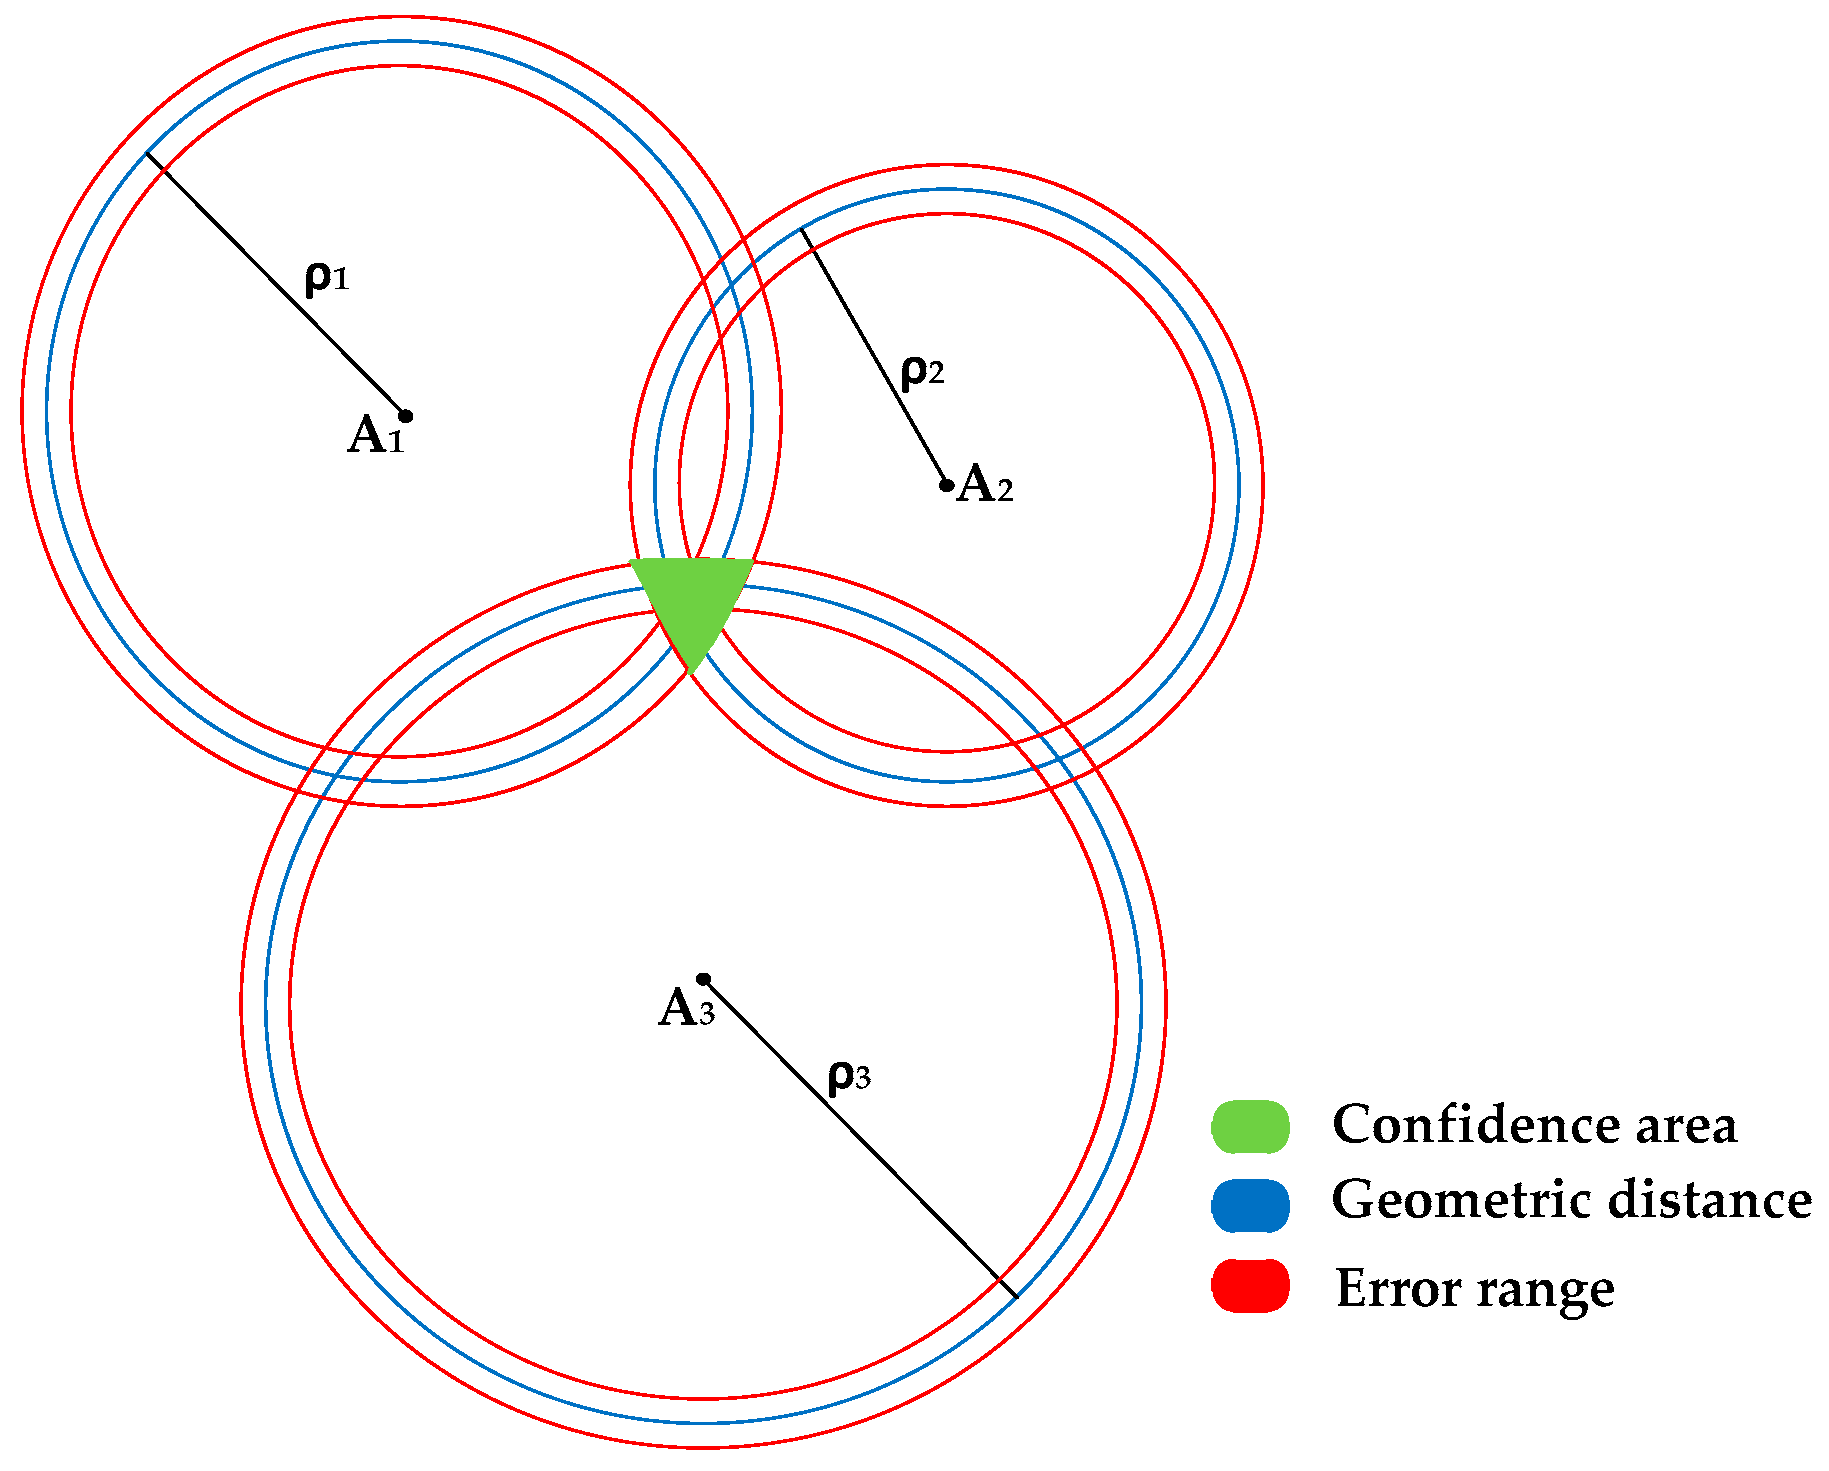
\includegraphics[width=0.6\textwidth]{pictures/multilateration/multilateration_error_ranges.png}
    \caption[Example of multilateration in 2D with error ranges]{
        An example of multilateration in 2D with error ranges.
        In contrast to the example shown in \Cref{pic:multilateration-gps-2d-3d-example}, the margins of error can be seen as well as the non-definite margin of error around the estimated device position~\protect\cite{kapoor_novel_2016}.
    }\label{pic:multilateration-with-error-ranges-example}
\end{figure}

When dealing with such inaccuracies, the calculated position of the device often is calculated as not a single point but a range of possible positions.

\Cref{pic:multilateration-with-error-ranges-example} shows an example of this in 2D where the device's position is estimated to be in the area where the three annuli (circles/``donuts'') overlap.
This does not result in a definite position of the device but rather a range of possible positions.
The accuracy of this estimated localization range depends on the accuracy of the distance measurements.

The following sections will explain different methods of determining the distance between a device and a receiver.
The accuracy of these distance measurements is crucial for the accuracy of the actual localization.

\subsubsection{Using \acl{ToA} to determine distances}\label{sec:toa-based-multilateration}

The \ac{ToA}-based method uses the difference in the signal's time of arrival at the receiving stations.
In conjunction with the speed of light ($299792458\ \mathrm{m/s}$), this time difference can be used to calculate the distance between the transmitter and receiver~\cite{khalaf-allah_time_2015}.

\ac{ToA} is being used by radio location systems like \ac{GPS} to determine the position of a device by using Multilateration~\cite{department_of_defense_usa_gps_2020}.
For GPS, usually four or more satellites are required to determine the position of a device accurately.

\ac{ToA} based multilateration requires the reference stations to be time-synchronized with each other in order to produce good results.
Since the speed of light is extremely high, even minor differences in time synchronization between reference points can result in significant inaccuracies in the calculated distance between them.

\subsubsection{Using the \acl{RSSI} to determine distances}\label{sec:rssi-based-multilateration}

This method uses the \acf{RSSI} values that were explained in \Cref{sec:rssi} to determine the distance between sender and receiver.
The distance between sender and receiver usually decreases in correlation with the measured \ac{RSSI} value as has been explained in \Cref{sec:background-free-space-path-loss}.
However, as mentioned in \Cref{sec:multipath-propagation}, the \ac{RSSI} value can be also affected by other factors like obstacles and the environment (\ac{MPP}).

These facts make \ac{RSSI}-based localization only work accurately in environments with little to no obstacles and thus a low amount of multipath propagation.
\Cref{sec:rssi-based-multilateration-implementation} will describe how this method was implemented in two different forms in this thesis.

\subsection{Fingerprinting with \acl{RSS} values}\label{sec:rssi-fingerprinting}

Another method for locating \aclp{ED} is through fingerprinting~\cite{xia_indoor_2017}.
This method utilizes a set of known locations with corresponding values to establish the location of \aclp{ED}.
The association of an input value with its corresponding location is called a fingerprint.
When a new set of input values is recorded by a device, these values are compared to the \ac{DB} of known fingerprints.
By performing similarity comparisons with the known fingerprints, the device's location can be estimated.
If multiple fingerprints match, the device's location can be estimated by calculating the average or center of the locations of the matching fingerprints.

For the purposes of this thesis, fingerprinting specifically relied on the \ac{RSS} values it receives from surrounding \aclp{LRWGW} as well as some other values.
The implementation of \ac{RSSI} fingerprinting for \ac{LoRaWAN} localization will be explained in \Cref{sec:fingerprinting-implementation}.
While \ac{ML} approaches can be used to improve fingerprinting, they were not used in this work, only simpler similarity calculations.

Fortunately, building a \ac{DB} of fingerprints for the use case explored in this thesis is fairly straightforward, since the \ac{TTNM} \ac{API} already provides the necessary raw data, as mentioned in \Cref{sec:ttn-mapper-importance}.
\Cref{sec:collecting-additional-ttnm-data} will explain the \aclp{LRWED} used to collect additional data for fingerprinting.

\subsubsection{Using additional values for the fingerprinting approach}\label{sec:fingerprinting-additional-values}

In addition to the \ac{RSS} values, other values were used in this thesis in an attempt to improve the accuracy of fingerprinting.
These values are the \ac{SNR} and the \ac{SF} of the received packets.
They are recorded by \ac{TTN} in addition to the \ac{RSS} values for each \acl{LRWGW} that received the packet, so it was simple to include them in the fingerprinting \ac{DB}.
Furthermore, \ac{TTNM} also has those additional parameters in its \ac{DB} that is accessible via the \ac{TTNM} \ac{API}.